\documentclass[11pt]{amsart}
\pdfsuppressptexinfo=-1
\usepackage[T1]{fontenc}
\usepackage{lmodern}
\usepackage[margin=1.1in]{geometry}
\usepackage{amsmath,amssymb,amsthm,mathtools}
\usepackage{booktabs,enumitem}
\usepackage{tikz}
\usepackage[hidelinks]{hyperref}

\newtheorem{theorem}{Theorem}[section]
\newtheorem{lemma}[theorem]{Lemma}
\newtheorem{proposition}[theorem]{Proposition}
\newtheorem{corollary}[theorem]{Corollary}
\theoremstyle{definition}
\newtheorem{definition}[theorem]{Definition}
\theoremstyle{remark}
\newtheorem{remark}[theorem]{Remark}
\numberwithin{equation}{section}
\setlength{\emergencystretch}{2em}
\raggedbottom

\newcommand{\R}{\mathbb{R}}
\newcommand{\area}{\operatorname{area}}
\newcommand{\conv}{\operatorname{conv}}
\newcommand{\lmin}{\lambda_{\min}}
% Certified values and certificate data (one place; Table 1 and the text use these macros).
\newcommand{\LBTHREE}{0.8347}
\newcommand{\LBFOUR}{0.836}
\newcommand{\LBFIVE}{0.8366}
\newcommand{\LBMAIN}{0.8366}
\newcommand{\NodesThree}{53{,}752}
\newcommand{\LeavesThree}{27{,}388}
\newcommand{\NodesFour}{1{,}552{,}274}
\newcommand{\LeavesFour}{808{,}905}
\newcommand{\DepthThree}{43}
\newcommand{\DepthFour}{50}
\newcommand{\WThree}{$0.193613$, $0.196856$}
\newcommand{\WFourTwo}{\begin{tabular}[t]{@{}l@{}}$0.198977$, $0.201023$,\\ $0.199964$\end{tabular}}
\newcommand{\MinLThree}{0.834700004923}
\newcommand{\MinLFour}{0.836000001625}
\newcommand{\RootMarginThree}{$4.0\times10^{-9}$}
\newcommand{\RootMarginFour}{$4.5\times10^{-9}$}
\newcommand{\SearchThree}{$308$\,s; $531$\,s}
\newcommand{\SearchFour}{$987$\,s; $8{,}728$\,s}
\newcommand{\CheckThree}{$95$\,s; $172$\,s}
\newcommand{\CheckFour}{$1{,}069$\,s; $9{,}786$\,s}
\newcommand{\IndepThree}{$451$ ($7$)}
\newcommand{\IndepFour}{$350$ ($7$)}
\newcommand{\IndepMarginThree}{$2.1\times10^{-5}$}
\newcommand{\IndepMarginFour}{$5.7\times10^{-4}$}
\newcommand{\NumMinCThree}{$0.8347836763$}
\newcommand{\NumMinLThree}{$0.8347809458$}
\newcommand{\NumMinCFour}{$0.8365614$}
\newcommand{\NumMinLFour}{$0.8364904560$}
\newcommand{\ArchThree}{$17{,}308$}
\newcommand{\ArchFour}{$487{,}316$}
\newcommand{\ShaThree}{2026ebe7e5339b89542e0429e5ad704b1a956278e3ae455b6d667b4c11892846}
\newcommand{\ShaFour}{d8a7f09dc236a7c647147bacc3e903f3c9e2bd2cadb601d000d1a67a2a237681}
% Certificate for D, B3, B5, B7, B9 (cert11d_08366).
\newcommand{\NodesFive}{32{,}384{,}756}
\newcommand{\LeavesFive}{16{,}193{,}402}
\newcommand{\MultiLeavesFive}{10{,}883{,}512}
\newcommand{\FarLeavesFive}{33}
\newcommand{\DepthFive}{73}
\newcommand{\MinLFive}{0.836600000032}
\newcommand{\RootMarginFive}{$3.0\times10^{-9}$}
\newcommand{\SearchFive}{$9{,}556$\,s; $2{,}847{,}069$\,s}
\newcommand{\CheckFive}{$5{,}286$\,s; $1{,}423{,}067$\,s}
\newcommand{\IndepFive}{$16{,}193{,}402$ ($9{,}018$)}
\newcommand{\IndepMarginFive}{$2.7\times10^{-3}$}
\newcommand{\NumMinCFive}{$0.8377599866$}
\newcommand{\NumMinLFive}{$0.8372950064$}
\newcommand{\ArchFive}{$293{,}113{,}544$}
\newcommand{\ShaFive}{6b5d28bc488edcfde9c6a49f3cb364f9086f445a58f85f166da23727036cf122}
\newcommand{\PartsFive}{$2{,}048$}
% Output of the first pass of the second verifier on cert11d_08366 (supplement archive).
\newcommand{\ArchPassOne}{$116{,}500{,}532$}
\newcommand{\ShaPassOne}{0cf9696eb47681382492bc547d44519beeb69f492ee0cf26c520ec8254e1562b}
% Lean proof (Section 4.6): archives of the generated modules and of their compiled files (supplement).
\newcommand{\ArchLeanSrc}{$133{,}521{,}541$}
\newcommand{\ShaLeanSrc}{acb85d373917295c26f77acd2b2144c2f47256fcc6d9418dface3ff78c00133a}
\newcommand{\ArchLeanOlean}{$481{,}071{,}638$}
\newcommand{\ShaLeanOlean}{9a356edf6e801783658a296ebe9f52430212006e4ee700c3be5a1b285f12dbab}
% Kernel-checked proof for D, B3, B5 (Section 4.6): its certificate and the archives of its generated modules.
\newcommand{\CellsK}{1{,}024}
\newcommand{\LeavesK}{25{,}214}
\newcommand{\ModulesK}{821}
\newcommand{\ArchKSrc}{$10{,}869{,}411$}
\newcommand{\ShaKSrc}{31a2058b782dab1dd5131267bf5a7e075bc343e963703bf684e1ed0c01235f4c}
\newcommand{\ArchKOlean}{$3{,}568{,}240{,}020$}
\newcommand{\ShaKOlean}{0caa58bf3ac7f5494053fe948dac88b16d08147c7a55e8334057196357e683e6}
% Kernel-checked proof for D, B3, B5, B7 (Section 4.6): its certificate and the archives of its generated modules.
\newcommand{\CellsKE}{65{,}536}
\newcommand{\LeavesKE}{278{,}093}
\newcommand{\ModulesKE}{9{,}034}
\newcommand{\ArchKESrc}{$1{,}155{,}309{,}716$}
\newcommand{\ShaKESrc}{3a0ff3ea18eb81b481f8a513ba632304af503f6140dfad6479317ec708491191}
\newcommand{\ArchKEOlean}{$936{,}081{,}748$}
\newcommand{\ShaKEOlean}{42091e9314c44daae000798e1bfb85365e00cc22bbb0a6ba73053f5535c5a70e}
% Kernel-checked proof for D, B3, B5, B7, B9 (Section 4.6).
\newcommand{\LeavesKEl}{9{,}239{,}121}
\newcommand{\CombLeavesKEl}{5{,}599{,}347}
\newcommand{\LeafModulesKEl}{331{,}762}
\newcommand{\ModulesKEl}{406{,}888}
\newcommand{\HoursKEl}{$83{,}000$}
\newcommand{\MemKEl}{$241$}
% Kernel-checked proof for D, B3, B5, B7, B9: archives of the cell modules, of the tree walks and of the hash lists.
\newcommand{\NTarsKEl}{sixteen}
\newcommand{\ArchKElSrc}{$29{,}879{,}869{,}440$}
\newcommand{\ArchKElGlue}{$66{,}701{,}378$}
\newcommand{\ShaKElGlue}{765203c48ea883ec00ce50b1fcc5a48adc9bf7da7e9f4741c3b8a89308faac6c}
\newcommand{\ArchKElSums}{$66{,}568{,}744$}
\newcommand{\ShaKElSums}{1b96415125a178a4c16014a9c7b96c272adc8e32f7ac03291d7d3d95a4aa5234}
% Release slots.
\newcommand{\ZENODODOI}{10.5281/zenodo.23717912}
\newcommand{\REPOURL}{https://github.com/tejasvi/lebesgue-cover-bound/tree/v9}
\hypersetup{pdftitle={A lower bound of \LBMAIN\ for Lebesgue's universal covering problem},
  pdfauthor={Tejasvi Singh Tomar}}

\begin{document}

\title[Lebesgue's universal covering problem]{A lower bound of \LBMAIN{} for Lebesgue's universal covering problem}
\author{Tejasvi Singh Tomar}
\renewcommand{\urladdrname}{{\itshape ORCID}}
\urladdr{\href{https://orcid.org/0000-0003-4668-3639}{https://orcid.org/0000-0003-4668-3639}}
\subjclass[2020]{52A10, 52A38; 65G40, 68V05, 68V20}
\keywords{Lebesgue's universal covering problem, Reuleaux polygons, convex hull, branch and bound, interval arithmetic, computer-assisted proof, formal verification, Lean 4}

\begin{abstract}
A universal cover is a convex set in the plane that contains a congruent copy of every set of diameter at most~$1$. Lebesgue asked in 1914 for a universal cover of least area; before this work, the infimum $\Lambda$ of the areas of universal covers was known to satisfy $0.83474\le\Lambda\le0.8441$. Lower bounds come from test sets: $\Lambda$ is bounded below by the least area of a convex hull of congruent copies of given sets of diameter at most~$1$. The best earlier lower bounds used the disk, the Reuleaux triangle and the Reuleaux pentagon, but these three bodies are known to admit a placement with hull area below $0.83479$, so they cannot give a much better bound. Adding the regular Reuleaux heptagon and nonagon of width~$1$, we improve the lower bound to $\Lambda\ge\LBMAIN$. Without the nonagon, the other four bodies already give $\Lambda\ge\LBFOUR$. The proof is a computer-assisted branch and bound over the relative placements of the bodies. Its certificates are checked in interval arithmetic, and separate proofs of both bounds in Lean~4, with their own certificates, are checked entirely by Lean's kernel.
\end{abstract}

\maketitle

\section{Introduction}\label{sec:intro}

A planar set has diameter at most~$1$ if any two of its points are at distance at most~$1$. A \emph{universal cover} is a convex set in the plane that contains a congruent copy of every planar set of diameter at most~$1$. In a letter of 1914 to Pál, Lebesgue asked for a universal cover of least area \cite{Pal20}. We write $\Lambda$ for the infimum of the areas of universal covers. Its value is not known \cite{BMP05}, and it is listed as constant 13b in the repository \emph{Optimization constants in mathematics} \cite{Tao26}.

Upper bounds come from explicit covers. Pál \cite{Pal20} proved that the regular hexagon circumscribed about a disk of diameter~$1$ is a universal cover. He then cut off two of its corners, which shows $\Lambda\le2-2/\sqrt3<0.8453$. Sprague \cite{Spr36}, Hansen \cite{Han92}, and Baez, Bagdasaryan and Gibbs \cite{BBG15} removed further small pieces. The best upper bound, $\Lambda\le0.8440935944$, is due to Gibbs \cite{Gib18}.

Lower bounds come from test sets. Let $T_1,\dots,T_m$ be sets of diameter at most~$1$. A universal cover contains a congruent copy of each $T_i$, and since it is convex, it contains the convex hull of these copies. Hence $\Lambda$ is at least the infimum $M(T_1,\dots,T_m)$ of the areas of such hulls (Lemma~\ref{lem:testsets}). Pál \cite{Pal20} took a disk and an equilateral triangle of diameter~$1$ and proved $\Lambda\ge\pi/8+\sqrt3/4>0.8257$.\footnote{The repository \cite{Tao26} credits $0.8257$ to Elekes \cite{Ele94}; we follow Mishra \cite[Section~1]{Mis26} in crediting it to Pál.} Elekes \cite{Ele94} took a disk and regular polygons whose numbers of sides are powers of~$3$ and proved $\Lambda\ge0.8271$. Brass and Sharifi \cite{BS05} took a disk, an equilateral triangle and a regular pentagon. They reduced the placements of these sets to a five-dimensional space, subdivided it, and proved $\Lambda\ge0.832$. Xie \cite{Xie26} certified $0.833$ for the same three sets with interval arithmetic. Gibbs \cite{Gib14} proposed sets of constant width as test sets, among them the regular Reuleaux $3$-, $5$-, $7$- and $9$-gons. Hatchett \cite{Hat26}, Mishra \cite{Mis26} and Zeng \cite{Zen26} used the disk with the Reuleaux triangle and pentagon of width~$1$, which contain the triangle and the pentagon. They proved $\Lambda\ge0.83474$, $\Lambda\ge0.8344$ and $\Lambda\ge0.834$, respectively. Mishra also gave a placement of these three bodies and proved, with a circumscribed polygon, that its hull has area at most $0.834781191$, so no lower bound obtained from them exceeds this value \cite[Section~3]{Mis26}.

Let $D$ be the disk of diameter~$1$, and let $B_n$ be the regular Reuleaux $n$-gon of width~$1$ (Definition~\ref{def:reuleaux}).

\begin{theorem}\label{thm:main}
We have
\[
M(D,B_3,B_5,B_7)\ge\LBFOUR\qquad\text{and}\qquad M(D,B_3,B_5,B_7,B_9)\ge\LBFIVE.
\]
Consequently $\Lambda\ge\LBFIVE$.
\end{theorem}

The sets $D$ and $B_n$ are convex, have diameter~$1$ and have an axis of symmetry. Therefore the bound $\Lambda\ge\LBFIVE$ holds whether or not congruent copies may be reflected, and whether a universal cover must contain copies of all sets of diameter at most~$1$ or only of the convex sets of diameter~$1$. Lemma~\ref{lem:testsets} does use the convexity of universal covers, which is part of their definition.

As a test of the method on the five-dimensional space of placements of $D$, $B_3$ and $B_5$, we also prove $M(D,B_3,B_5)\ge\LBTHREE$ (Proposition~\ref{prop:five}). Its target lies slightly below Hatchett's bound $0.83474$, and Section~\ref{sec:limits} compares the two certificates. In the certificates of Section~\ref{sec:cert}, the bounds for three and for four bodies use the Taylor bound of Lemma~\ref{lem:taylor} alone; only the bound for five bodies also combines the areas of several polygons (Lemma~\ref{lem:comb}).

Local minimization finds placements of the four and of the five bodies with hull areas of about $0.83649$ and $0.83730$ (Section~\ref{sec:limits}). Every placement bounds the least hull area from above. These two values are computed in floating point and are not certified; up to floating-point error, lower bounds from these bodies cannot go beyond them.

\subsection*{The method}
We fix the disk and the rotation of the Reuleaux triangle; a placement of the bodies is then a point $p$ of $\R^5$, $\R^8$ or $\R^{11}$. Let $A(p)$ be the area of the convex hull of the placed bodies, and let $\tau$ be the target, the bound to be proved. If the centre of a Reuleaux polygon is more than about $0.2$ from the centre of the disk, a safe rather than a sharp distance, the hull of these two bodies already has area larger than $\tau$. The angles can be restricted by the rotational symmetries of the bodies and by the reflection of the whole placement in a line through the centre of the disk parallel to an axis of symmetry of the Reuleaux triangle. So it suffices to show $A>\tau$ on a box $X$ of placements (Section~\ref{sec:reduction}), and we do this by a branch and bound over subboxes of $X$. Bounds for $A$ on a box that use no derivatives lose an amount proportional to the width of the box even where $A$ hardly varies \cite{Mis26,Xie26}, and the first-order bounds of \cite{Hat26,Zen26} bound the second-order remainder by absolute values of second derivatives. Near a minimizing placement, where $A$ exceeds the target by little, both need very small boxes. Mishra found the four bodies $D,B_3,B_5,B_7$ out of reach for his method (Section~\ref{sec:limits}).

On a box of placements we replace the hull by a polygon inside it, as in Figure~\ref{fig:placement}. For each box, the vertices of the polygon are computed for the placement $c$ at the centre of the box, as support points of the hull in many directions (Section~\ref{sec:search}). Once chosen, each vertex moves with its body. If, on the whole box, the vertices stay in strict angular order around a point $z$ of the disk chosen for the box, then the area $F$ of the polygon through them, in this order, is at most $A$ (Lemma~\ref{lem:fanbox}). Since each vertex moves rigidly with its body, $F$ is a polynomial in the translations and in the sines and cosines of the angles. On the box we bound $F$ from below through its value and gradient at $c$ and a certified lower bound for the smallest eigenvalue of its Hessian, together with a bound for how much the Hessian varies over the box. Near placements where the combinatorial type of the hull changes, that is, where the corners and arcs that form its boundary change, the certificate for the five bodies bounds instead a convex combination of the areas of several such polygons, weighted so that their gradients at $c$ nearly cancel.

\begin{figure}[t]
\centering
% Figure 1: the placement of independent/opt11_point.json and a witness fan whose witnesses are the support points
% of the hull in 48 equally spaced directions; each arc of a Reuleaux polygon is drawn exactly.
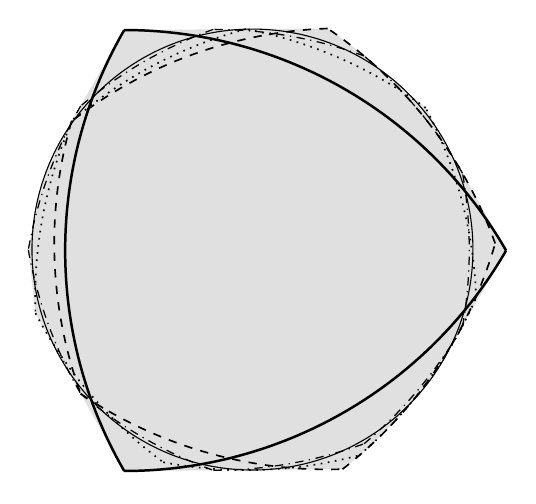
\begin{tikzpicture}[x=5.6cm,y=5.6cm]
\fill[black!12] (-0.5083,-0.0007) -- (-0.4921,-0.1445) -- (-0.4921,-0.1445) -- (-0.4901,-0.1481) -- (-0.4882,-0.1517) -- (-0.4862,-0.1554) -- (-0.4843,-0.1590) -- (-0.4823,-0.1626) -- (-0.4803,-0.1662) -- (-0.4783,-0.1698) -- (-0.3946,-0.3182) -- (-0.3896,-0.3271) -- (-0.2960,-0.4931) -- (-0.2938,-0.4969) -- (-0.2917,-0.5007) -- (-0.2908,-0.5022) -- (-0.2864,-0.5022) -- (-0.0812,-0.5006) -- (-0.0071,-0.5001) -- (0.1781,-0.4987) -- (0.1823,-0.4986) -- (0.1865,-0.4986) -- (0.1907,-0.4985) -- (0.1949,-0.4984) -- (0.1991,-0.4983) -- (0.2032,-0.4982) -- (0.2043,-0.4981) -- (0.2076,-0.4956) -- (0.2109,-0.4930) -- (0.2142,-0.4903) -- (0.2174,-0.4877) -- (0.2207,-0.4851) -- (0.2239,-0.4824) -- (0.2272,-0.4798) -- (0.2304,-0.4771) -- (0.2336,-0.4744) -- (0.2368,-0.4717) -- (0.2400,-0.4690) -- (0.2431,-0.4663) -- (0.2463,-0.4635) -- (0.2495,-0.4608) -- (0.2526,-0.4580) -- (0.2557,-0.4552) -- (0.2589,-0.4524) -- (0.2620,-0.4496) -- (0.2651,-0.4468) -- (0.2681,-0.4439) -- (0.2712,-0.4411) -- (0.2743,-0.4382) -- (0.2773,-0.4353) -- (0.2803,-0.4325) -- (0.2834,-0.4296) -- (0.2864,-0.4266) -- (0.2894,-0.4237) -- (0.2924,-0.4208) -- (0.2953,-0.4178) -- (0.2983,-0.4149) -- (0.3013,-0.4119) -- (0.3042,-0.4089) -- (0.3071,-0.4059) -- (0.3100,-0.4029) -- (0.3129,-0.3999) -- (0.3158,-0.3968) -- (0.3187,-0.3938) -- (0.3215,-0.3907) -- (0.3244,-0.3877) -- (0.3271,-0.3847) -- (0.3299,-0.3817) -- (0.3327,-0.3786) -- (0.3354,-0.3756) -- (0.3382,-0.3725) -- (0.3409,-0.3694) -- (0.3751,-0.3307) -- (0.3782,-0.3271) -- (0.3812,-0.3235) -- (0.3843,-0.3199) -- (0.3873,-0.3163) -- (0.3902,-0.3126) -- (0.3931,-0.3089) -- (0.3960,-0.3052) -- (0.3989,-0.3015) -- (0.4017,-0.2977) -- (0.4045,-0.2939) -- (0.4073,-0.2901) -- (0.4100,-0.2862) -- (0.4127,-0.2823) -- (0.4153,-0.2784) -- (0.4179,-0.2745) -- (0.4205,-0.2706) -- (0.4230,-0.2666) -- (0.4255,-0.2626) -- (0.4280,-0.2586) -- (0.4304,-0.2545) -- (0.4328,-0.2505) -- (0.4588,-0.2050) -- (0.4765,-0.1743) -- (0.5752,-0.0022) -- (0.4765,0.1730) -- (0.3929,0.3212) -- (0.3271,0.3782) -- (0.3235,0.3812) -- (0.3199,0.3843) -- (0.2532,0.4390) -- (0.2449,0.4459) -- (0.2416,0.4485) -- (0.2384,0.4512) -- (0.2351,0.4538) -- (0.2318,0.4564) -- (0.2285,0.4590) -- (0.2252,0.4616) -- (0.2219,0.4642) -- (0.2186,0.4667) -- (0.2153,0.4693) -- (0.2119,0.4718) -- (0.2086,0.4743) -- (0.2052,0.4768) -- (0.2019,0.4793) -- (0.1985,0.4818) -- (0.1951,0.4842) -- (0.1917,0.4867) -- (0.1883,0.4891) -- (0.1848,0.4915) -- (0.1814,0.4939) -- (0.1780,0.4963) -- (0.1745,0.4986) -- (0.1710,0.5010) -- (0.1706,0.5013) -- (-0.2908,0.4978) -- (-0.2908,0.4978) -- (-0.4104,0.2906) -- (-0.4366,0.2436) -- (-0.4389,0.2395) -- (-0.4411,0.2354) -- (-0.4433,0.2312) -- (-0.4455,0.2270) -- (-0.4476,0.2228) -- (-0.4497,0.2186) -- (-0.4517,0.2143) -- (-0.4537,0.2100) -- (-0.4557,0.2058) -- (-0.4576,0.2015) -- (-0.4595,0.1971) -- (-0.4613,0.1928) -- (-0.4631,0.1884) -- (-0.4649,0.1841) -- (-0.4666,0.1797) -- (-0.4683,0.1753) -- (-0.4699,0.1708) -- (-0.4715,0.1664) -- (-0.4730,0.1620) -- (-0.4745,0.1575) -- (-0.4760,0.1530) -- (-0.4774,0.1485) -- (-0.4788,0.1440) -- (-0.4801,0.1395) -- (-0.4814,0.1350) -- (-0.4827,0.1304) -- (-0.4839,0.1259) -- (-0.4851,0.1213) -- (-0.4862,0.1167) -- (-0.4873,0.1121) -- (-0.4883,0.1075) -- (-0.4893,0.1029) -- (-0.4902,0.0983) -- (-0.4911,0.0937) -- (-0.5073,0.0051) -- (-0.5080,0.0011) -- (-0.5083,-0.0007) -- cycle;
\draw[line width=0.4pt] (0,0) circle[radius=0.5];
\draw[line width=0.9pt] (-0.29079,0.49783) arc[start angle=150.0000, end angle=210.0000, radius=1];
\draw[line width=0.9pt] (-0.29079,-0.50217) arc[start angle=-90.0000, end angle=-30.0000, radius=1];
\draw[line width=0.9pt] (0.57523,-0.00217) arc[start angle=30.0000, end angle=90.0000, radius=1];
\draw[line width=0.6pt, dashed] (-0.41041,0.29063) arc[start angle=163.9300, end angle=199.9300, radius=1];
\draw[line width=0.6pt, dashed] (-0.38959,-0.32706) arc[start angle=-124.0700, end angle=-88.0700, radius=1];
\draw[line width=0.6pt, dashed] (0.20429,-0.49814) arc[start angle=-52.0700, end angle=-16.0700, radius=1];
\draw[line width=0.6pt, dashed] (0.55052,0.01381) arc[start angle=19.9300, end angle=55.9300, radius=1];
\draw[line width=0.6pt, dashed] (0.17061,0.50130) arc[start angle=91.9300, end angle=127.9300, radius=1];
\draw[line width=0.6pt, dotted] (-0.49206,-0.14448) arc[start angle=-152.2449, end angle=-126.5306, radius=1];
\draw[line width=0.6pt, dotted] (-0.20236,-0.48233) arc[start angle=-100.8164, end angle=-75.1021, radius=1];
\draw[line width=0.6pt, dotted] (0.24240,-0.46648) arc[start angle=-49.3878, end angle=-23.6735, radius=1];
\draw[line width=0.6pt, dotted] (0.50731,-0.10887) arc[start angle=2.0408, end angle=27.7551, radius=1];
\draw[line width=0.6pt, dotted] (0.39289,0.32121) arc[start angle=53.4694, end angle=79.1836, radius=1];
\draw[line width=0.6pt, dotted] (-0.01470,0.49990) arc[start angle=104.8979, end angle=130.6122, radius=1];
\draw[line width=0.6pt, dotted] (-0.40854,0.29265) arc[start angle=156.3265, end angle=182.0408, radius=1];
\draw[line width=0.45pt, dash dot] (-0.50835,-0.00066) arc[start angle=-169.9984, end angle=-149.9984, radius=1];
\draw[line width=0.45pt, dash dot] (-0.38956,-0.32701) arc[start angle=-129.9984, end angle=-109.9984, radius=1];
\draw[line width=0.45pt, dash dot] (-0.08878,-0.50065) arc[start angle=-89.9984, end angle=-69.9984, radius=1];
\draw[line width=0.45pt, dash dot] (0.25323,-0.44034) arc[start angle=-49.9984, end angle=-29.9984, radius=1];
\draw[line width=0.45pt, dash dot] (0.47646,-0.17429) arc[start angle=-9.9984, end angle=10.0016, radius=1];
\draw[line width=0.45pt, dash dot] (0.47645,0.17301) arc[start angle=30.0016, end angle=50.0016, radius=1];
\draw[line width=0.45pt, dash dot] (0.25321,0.43905) arc[start angle=70.0016, end angle=90.0016, radius=1];
\draw[line width=0.45pt, dash dot] (-0.08881,0.49935) arc[start angle=110.0016, end angle=130.0016, radius=1];
\draw[line width=0.45pt, dash dot] (-0.38958,0.32569) arc[start angle=150.0016, end angle=170.0016, radius=1];
\end{tikzpicture}\hfill
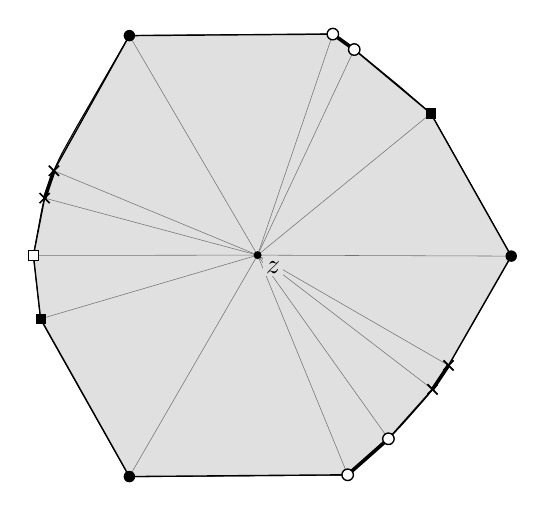
\begin{tikzpicture}[x=5.6cm,y=5.6cm]
\draw[line width=0.4pt] (-0.5083,-0.0007) -- (-0.4921,-0.1445) -- (-0.4921,-0.1445) -- (-0.4901,-0.1481) -- (-0.4882,-0.1517) -- (-0.4862,-0.1554) -- (-0.4843,-0.1590) -- (-0.4823,-0.1626) -- (-0.4803,-0.1662) -- (-0.4783,-0.1698) -- (-0.3946,-0.3182) -- (-0.3896,-0.3271) -- (-0.2960,-0.4931) -- (-0.2938,-0.4969) -- (-0.2917,-0.5007) -- (-0.2908,-0.5022) -- (-0.2864,-0.5022) -- (-0.0812,-0.5006) -- (-0.0071,-0.5001) -- (0.1781,-0.4987) -- (0.1823,-0.4986) -- (0.1865,-0.4986) -- (0.1907,-0.4985) -- (0.1949,-0.4984) -- (0.1991,-0.4983) -- (0.2032,-0.4982) -- (0.2043,-0.4981) -- (0.2076,-0.4956) -- (0.2109,-0.4930) -- (0.2142,-0.4903) -- (0.2174,-0.4877) -- (0.2207,-0.4851) -- (0.2239,-0.4824) -- (0.2272,-0.4798) -- (0.2304,-0.4771) -- (0.2336,-0.4744) -- (0.2368,-0.4717) -- (0.2400,-0.4690) -- (0.2431,-0.4663) -- (0.2463,-0.4635) -- (0.2495,-0.4608) -- (0.2526,-0.4580) -- (0.2557,-0.4552) -- (0.2589,-0.4524) -- (0.2620,-0.4496) -- (0.2651,-0.4468) -- (0.2681,-0.4439) -- (0.2712,-0.4411) -- (0.2743,-0.4382) -- (0.2773,-0.4353) -- (0.2803,-0.4325) -- (0.2834,-0.4296) -- (0.2864,-0.4266) -- (0.2894,-0.4237) -- (0.2924,-0.4208) -- (0.2953,-0.4178) -- (0.2983,-0.4149) -- (0.3013,-0.4119) -- (0.3042,-0.4089) -- (0.3071,-0.4059) -- (0.3100,-0.4029) -- (0.3129,-0.3999) -- (0.3158,-0.3968) -- (0.3187,-0.3938) -- (0.3215,-0.3907) -- (0.3244,-0.3877) -- (0.3271,-0.3847) -- (0.3299,-0.3817) -- (0.3327,-0.3786) -- (0.3354,-0.3756) -- (0.3382,-0.3725) -- (0.3409,-0.3694) -- (0.3751,-0.3307) -- (0.3782,-0.3271) -- (0.3812,-0.3235) -- (0.3843,-0.3199) -- (0.3873,-0.3163) -- (0.3902,-0.3126) -- (0.3931,-0.3089) -- (0.3960,-0.3052) -- (0.3989,-0.3015) -- (0.4017,-0.2977) -- (0.4045,-0.2939) -- (0.4073,-0.2901) -- (0.4100,-0.2862) -- (0.4127,-0.2823) -- (0.4153,-0.2784) -- (0.4179,-0.2745) -- (0.4205,-0.2706) -- (0.4230,-0.2666) -- (0.4255,-0.2626) -- (0.4280,-0.2586) -- (0.4304,-0.2545) -- (0.4328,-0.2505) -- (0.4588,-0.2050) -- (0.4765,-0.1743) -- (0.5752,-0.0022) -- (0.4765,0.1730) -- (0.3929,0.3212) -- (0.3271,0.3782) -- (0.3235,0.3812) -- (0.3199,0.3843) -- (0.2532,0.4390) -- (0.2449,0.4459) -- (0.2416,0.4485) -- (0.2384,0.4512) -- (0.2351,0.4538) -- (0.2318,0.4564) -- (0.2285,0.4590) -- (0.2252,0.4616) -- (0.2219,0.4642) -- (0.2186,0.4667) -- (0.2153,0.4693) -- (0.2119,0.4718) -- (0.2086,0.4743) -- (0.2052,0.4768) -- (0.2019,0.4793) -- (0.1985,0.4818) -- (0.1951,0.4842) -- (0.1917,0.4867) -- (0.1883,0.4891) -- (0.1848,0.4915) -- (0.1814,0.4939) -- (0.1780,0.4963) -- (0.1745,0.4986) -- (0.1710,0.5010) -- (0.1706,0.5013) -- (-0.2908,0.4978) -- (-0.2908,0.4978) -- (-0.4104,0.2906) -- (-0.4366,0.2436) -- (-0.4389,0.2395) -- (-0.4411,0.2354) -- (-0.4433,0.2312) -- (-0.4455,0.2270) -- (-0.4476,0.2228) -- (-0.4497,0.2186) -- (-0.4517,0.2143) -- (-0.4537,0.2100) -- (-0.4557,0.2058) -- (-0.4576,0.2015) -- (-0.4595,0.1971) -- (-0.4613,0.1928) -- (-0.4631,0.1884) -- (-0.4649,0.1841) -- (-0.4666,0.1797) -- (-0.4683,0.1753) -- (-0.4699,0.1708) -- (-0.4715,0.1664) -- (-0.4730,0.1620) -- (-0.4745,0.1575) -- (-0.4760,0.1530) -- (-0.4774,0.1485) -- (-0.4788,0.1440) -- (-0.4801,0.1395) -- (-0.4814,0.1350) -- (-0.4827,0.1304) -- (-0.4839,0.1259) -- (-0.4851,0.1213) -- (-0.4862,0.1167) -- (-0.4873,0.1121) -- (-0.4883,0.1075) -- (-0.4893,0.1029) -- (-0.4902,0.0983) -- (-0.4911,0.0937) -- (-0.5073,0.0051) -- (-0.5080,0.0011) -- (-0.5083,-0.0007) -- cycle;
\fill[black!12] (0.57523,-0.00217) -- (0.39289,0.32121) -- (0.21917,0.46630) -- (0.17061,0.50130) -- (-0.29079,0.49783) -- (-0.46194,0.19134) -- (-0.48296,0.12941) -- (-0.50835,-0.00066) -- (-0.49206,-0.14448) -- (-0.29079,-0.50217) -- (0.20429,-0.49814) -- (0.29670,-0.41648) -- (0.39668,-0.30438) -- (0.43301,-0.25000) -- cycle;
\draw[line width=0.2pt, black!55] (0,0) -- (0.57523,-0.00217);
\draw[line width=0.2pt, black!55] (0,0) -- (0.39289,0.32121);
\draw[line width=0.2pt, black!55] (0,0) -- (0.21917,0.46630);
\draw[line width=0.2pt, black!55] (0,0) -- (0.17061,0.50130);
\draw[line width=0.2pt, black!55] (0,0) -- (-0.29079,0.49783);
\draw[line width=0.2pt, black!55] (0,0) -- (-0.46194,0.19134);
\draw[line width=0.2pt, black!55] (0,0) -- (-0.48296,0.12941);
\draw[line width=0.2pt, black!55] (0,0) -- (-0.50835,-0.00066);
\draw[line width=0.2pt, black!55] (0,0) -- (-0.49206,-0.14448);
\draw[line width=0.2pt, black!55] (0,0) -- (-0.29079,-0.50217);
\draw[line width=0.2pt, black!55] (0,0) -- (0.20429,-0.49814);
\draw[line width=0.2pt, black!55] (0,0) -- (0.29670,-0.41648);
\draw[line width=0.2pt, black!55] (0,0) -- (0.39668,-0.30438);
\draw[line width=0.2pt, black!55] (0,0) -- (0.43301,-0.25000);
\draw[line width=0.5pt] (0.57523,-0.00217) -- (0.39289,0.32121);
\draw[line width=0.5pt] (0.39289,0.32121) -- (0.21917,0.46630);
\draw[line width=1.3pt] (0.21917,0.46630) -- (0.17061,0.50130);
\draw[line width=0.5pt] (0.17061,0.50130) -- (-0.29079,0.49783);
\draw[line width=0.5pt] (-0.29079,0.49783) -- (-0.46194,0.19134);
\draw[line width=1.3pt] (-0.46194,0.19134) -- (-0.48296,0.12941);
\draw[line width=0.5pt] (-0.48296,0.12941) -- (-0.50835,-0.00066);
\draw[line width=0.5pt] (-0.50835,-0.00066) -- (-0.49206,-0.14448);
\draw[line width=0.5pt] (-0.49206,-0.14448) -- (-0.29079,-0.50217);
\draw[line width=0.5pt] (-0.29079,-0.50217) -- (0.20429,-0.49814);
\draw[line width=1.3pt] (0.20429,-0.49814) -- (0.29670,-0.41648);
\draw[line width=0.5pt] (0.29670,-0.41648) -- (0.39668,-0.30438);
\draw[line width=1.3pt] (0.39668,-0.30438) -- (0.43301,-0.25000);
\draw[line width=0.5pt] (0.43301,-0.25000) -- (0.57523,-0.00217);
\fill (0.57523,-0.00217) circle[radius=0.013];
\fill (0.38139,0.30971) rectangle (0.40439,0.33271);
\filldraw[fill=white, line width=0.5pt] (0.21917,0.46630) circle[radius=0.013];
\filldraw[fill=white, line width=0.5pt] (0.17061,0.50130) circle[radius=0.013];
\fill (-0.29079,0.49783) circle[radius=0.013];
\draw[line width=0.6pt] (-0.47344,0.17984) -- (-0.45044,0.20284) (-0.47344,0.20284) -- (-0.45044,0.17984);
\draw[line width=0.6pt] (-0.49446,0.11791) -- (-0.47146,0.14091) (-0.49446,0.14091) -- (-0.47146,0.11791);
\filldraw[fill=white, line width=0.5pt] (-0.51985,-0.01216) rectangle (-0.49685,0.01084);
\fill (-0.50356,-0.15598) rectangle (-0.48056,-0.13298);
\fill (-0.29079,-0.50217) circle[radius=0.013];
\filldraw[fill=white, line width=0.5pt] (0.20429,-0.49814) circle[radius=0.013];
\filldraw[fill=white, line width=0.5pt] (0.29670,-0.41648) circle[radius=0.013];
\draw[line width=0.6pt] (0.38518,-0.31588) -- (0.40818,-0.29288) (0.38518,-0.29288) -- (0.40818,-0.31588);
\draw[line width=0.6pt] (0.42151,-0.26150) -- (0.44451,-0.23850) (0.42151,-0.23850) -- (0.44451,-0.26150);
\fill (0,0) circle[radius=0.009];
\node[anchor=north west, inner sep=1pt, fill=black!12] at (0.012,-0.006) {$z$};
\end{tikzpicture}
\caption{Left: the disk $D$ (thin) and the Reuleaux polygons $B_3$ (solid), $B_5$ (dashed), $B_7$ (dotted) and $B_9$ (dash-dotted) at the placement of Section~\ref{sec:limits}, found by local minimization; their convex hull, shaded, has area about $0.83730$. Right: a polygon inside this hull, of the kind used in Section~\ref{sec:box} (a witness fan), with $z$ the centre of the disk. Its vertices, the witnesses, are the $14$ distinct support points of the hull in $48$ equally spaced directions; a corner is the support point for many directions. They lie on $D$ ($\times$), $B_3$ ($\bullet$), $B_5$ ($\circ$), $B_7$ ($\blacksquare$) and $B_9$ ($\square$). A block of consecutive witnesses on one body is a run, and thick edges join its witnesses. The shaded polygon has area $F\approx0.83564$, about $0.0017$ less than the hull, so this coarse fan only illustrates the construction; the fans of the certificates use $256$ or $1024$ directions and further support points (Section~\ref{sec:search}).}\label{fig:placement}
\end{figure}

\subsection*{Outline}
Section~\ref{sec:reduction} reduces the problem to a box of placements, and Section~\ref{sec:box} proves the bounds on boxes. Section~\ref{sec:cert} describes the certificates and their checks. A checker that shares no code with the search program verifies all three certificates in ball arithmetic, a form of interval arithmetic, with the Arb library \cite{Joh17}; it relies on the lemmas of Sections~\ref{sec:reduction} and~\ref{sec:box}. Section~\ref{sec:lean} describes separate proofs of the bounds of Theorem~\ref{thm:main} and Proposition~\ref{prop:five} in Lean~4, with their own bound on boxes and their own certificates, and Lean's kernel checks these proofs. Section~\ref{sec:limits} discusses how far lower bounds from these test sets can go.

\section{Reduction to a box of placements}\label{sec:reduction}

We first fix notation. For $a,b\in\R^2$ put $\det(a,b)=a_1b_2-a_2b_1$. Let $u(\varphi)=(\cos\varphi,\sin\varphi)$, let $R_\varphi$ be the rotation of $\R^2$ about the origin by the angle $\varphi$, and let $J=R_{\pi/2}$. Rotations preserve $\det$, and $J$ commutes with every $R_\varphi$. Let $D(y,r)$ be the closed disk with centre $y$ and radius $r$, and let $D=D(0,1/2)$. We write $\area$ for the Lebesgue measure on $\R^2$, $\conv$ for the convex hull, and $|\cdot|$ for the Euclidean norm.

\begin{definition}\label{def:reuleaux}
For odd $n\ge3$ let $R_n=1/(2\cos(\pi/(2n)))$, let $V_{n,l}=R_n\,u(2\pi l/n)$ for $l=0,\dots,n-1$, and let $B_n=\bigcap_{l=0}^{n-1}D(V_{n,l},1)$.
\end{definition}

The points $V_{n,l}$ are the vertices of a regular $n$-gon. The largest distance between two of them is $|V_{n,0}-V_{n,(n-1)/2}|=2R_n\cos(\pi/(2n))=1$. Hence $B_n$ is the regular Reuleaux $n$-gon of width~$1$. It has constant width~$1$, and hence diameter~$1$ \cite{MMO19}. We have $0.50<R_9<R_7<R_5<R_3<0.58$.

We fix odd integers $n_1,\dots,n_k\ge3$ with $k\ge2$. Theorem~\ref{thm:main} uses $(n_1,n_2,n_3)=(3,5,7)$ and $(n_1,\dots,n_4)=(3,5,7,9)$, and Proposition~\ref{prop:five} uses $(n_1,n_2)=(3,5)$. A \emph{placement} is a vector
\[
p=(t_1,\rho_2,t_2,\dots,\rho_k,t_k)\in\R^d,\qquad d=3k-1,
\]
with $t_i\in\R^2$ and $\rho_i\in\R$. We put $\rho_1=0$, and for the disk we put $\rho_0=0$ and $t_0=0$. Let $B^{(0)}=D$ and $B^{(i)}=B_{n_i}$ for $1\le i\le k$. In the placement $p$, body $i$ occupies $P_i(p)=R_{\rho_i}B^{(i)}+t_i$. Let
\[
K(p)=\conv\bigl(P_0(p)\cup P_1(p)\cup\dots\cup P_k(p)\bigr)\qquad\text{and}\qquad A(p)=\area K(p).
\]
For bounded sets $T_1,\dots,T_m\subset\R^2$ let $M(T_1,\dots,T_m)$ be the infimum of $\area\conv(g_1(T_1)\cup\dots\cup g_m(T_m))$ over all isometries $g_1,\dots,g_m$ of $\R^2$.

Lemma~\ref{lem:testsets} below is the principle behind all the lower bounds above. Its normalization of the placements is that of Brass and Sharifi \cite{BS05} (see also \cite[Lemma~4.3]{Mis26}).

\begin{lemma}\label{lem:testsets}
If $T_1,\dots,T_m$ are planar sets of diameter at most~$1$, then $\Lambda\ge M(T_1,\dots,T_m)$. Moreover, $M(D,B_{n_1},\dots,B_{n_k})=\inf_{p\in\R^d}A(p)$.
\end{lemma}

\begin{proof}
Let $\Omega$ be a universal cover. For each $i$ there is an isometry $g_i$ with $g_i(T_i)\subseteq\Omega$. Since $\Omega$ is convex, it contains $\conv\bigl(\bigcup_ig_i(T_i)\bigr)$, so $\area\Omega\ge M(T_1,\dots,T_m)$. Taking the infimum over $\Omega$ proves the first claim.

Every placement is given by isometries, so $M(D,B_{n_1},\dots,B_{n_k})\le\inf A$. Conversely, let $g_0,\dots,g_k$ be isometries. The reflection $S(y_1,y_2)=(y_1,-y_2)$ maps $D$ to itself and permutes the points $V_{n,l}$, so it maps each $B^{(i)}$ to itself. If $g_i$ reverses orientation, we replace it by $g_i\circ S$, which preserves orientation and has the same image of $B^{(i)}$. So we may assume that $g_i(y)=R_{\alpha_i}y+b_i$ for all $i$. The rigid motion $h(y)=R_{-\alpha_1}(y-b_0)$ satisfies $h\circ g_i(y)=R_{\alpha_i-\alpha_1}y+R_{-\alpha_1}(b_i-b_0)$. Since $D$ is invariant under rotations about the origin, $h$ maps $g_i(B^{(i)})$ onto $P_i(p)$ for all $i$, where $p$ is the placement with $\rho_i=\alpha_i-\alpha_1$ and $t_i=R_{-\alpha_1}(b_i-b_0)$. As $h$ preserves areas, the hull of $g_0(B^{(0)}),\dots,g_k(B^{(k)})$ has area $A(p)\ge\inf A$.
\end{proof}

\begin{lemma}[Symmetry]\label{lem:symmetry}
For a placement $p$ let $\bar p=(St_1,-\rho_2,St_2,\dots,-\rho_k,St_k)$. Then $A(\bar p)=A(p)$. Moreover, $A$ is periodic in $\rho_i$ with period $2\pi/n_i$ for $2\le i\le k$. Consequently, $\inf A$ equals the infimum of $A$ over the placements with $0\le\rho_2\le\pi/n_2$ and $0\le\rho_i\le2\pi/n_i$ for $3\le i\le k$, and the reduction does not change $|t_1|,\dots,|t_k|$.
\end{lemma}

\begin{proof}
The reflection $S$ of the previous proof satisfies $S\circ R_\varphi=R_{-\varphi}\circ S$ and $S(B^{(i)})=B^{(i)}$. Hence $S(P_i(p))=R_{-\rho_i}B^{(i)}+St_i=P_i(\bar p)$ for all $i$. So $S(K(p))=K(\bar p)$, and $S$ preserves area. The rotation $R_{2\pi/n}$ permutes the points $V_{n,l}$, so $R_{2\pi/n}B_n=B_n$, and this gives the periodicity. Given a placement, we first shift $\rho_2$ into $[0,2\pi/n_2)$. If then $\rho_2>\pi/n_2$, we pass to $\bar p$ and shift its second coordinate $-\rho_2$ by $2\pi/n_2$ into $(0,\pi/n_2)$. Finally we shift $\rho_3,\dots,\rho_k$ into the intervals $[0,2\pi/n_i)$. None of these steps changes $|t_1|,\dots,|t_k|$.
\end{proof}

The next lemma gives the root box used by Brass and Sharifi \cite{BS05}. In this form, with the area $f$, it is in \cite[Lemma~4.4 and Remark~4.6]{Mis26}. Zeng \cite[Sections~S10.2 and~S10.3]{Zen26} and Hatchett \cite{Hat26} prove the same estimate for $B_3$ and $B_5$.

\begin{lemma}[Corner lemma]\label{lem:corner}
For $s\ge1/2$ and $m\ge0$ let
\[
f(s)=\frac{\pi-\arccos(1/(2s))}{4}+\frac{\sqrt{s^2-1/4}}{2}\qquad\text{and}\qquad g_n(m)=\sqrt{R_n^2+m^2+2R_nm\cos(\pi/n)}.
\]
Then $f$ and $g_n$ are increasing, $g_n(m)\ge R_n>1/2$, and $A(p)\ge f(g_{n_i}(|t_i|))$ for every placement $p$ and every $1\le i\le k$.
\end{lemma}

\begin{proof}
A direct computation gives $f'(s)=\sqrt{4s^2-1}/(4s)>0$ for $s>1/2$. Since $\cos(\pi/n)>0$, $g_n$ is increasing, and $g_n(0)=R_n>1/2$ because $\cos(\pi/(2n))<1$. Fix $i\ge1$ and write $n=n_i$, $\rho=\rho_i$ and $t=t_i$. The corners $y_l=R_\rho V_{n,l}+t$ lie in $P_i(p)$. If $t=0$, then $|y_l|=R_n=g_n(0)$. Otherwise we write $t=|t|\,u(\psi)$. The directions $\rho+2\pi l/n$ of the vectors $R_\rho V_{n,l}$ are spaced by $2\pi/n$, so for some $l$ the angle $\beta$ between $u(\rho+2\pi l/n)$ and $u(\psi)$ satisfies $\beta\le\pi/n$. For this $l$,
\[
|y_l|^2=R_n^2+|t|^2+2R_n|t|\cos\beta\ge g_n(|t|)^2.
\]
So $K(p)$ contains $D$ and a point $y$ with $s=|y|\ge g_n(|t|)>1/2$. The set $\conv(D\cup\{y\})$ is the union of two pieces. The first is the quadrilateral bounded by the two tangent segments from $y$ to $D$ and the two radii to their points of contact, of area $\frac12\sqrt{s^2-1/4}$. The second is the sector of $D$ outside this quadrilateral, of angle $2\pi-2\arccos(1/(2s))$ and area $(\pi-\arccos(1/(2s)))/4$. Hence $A(p)\ge f(s)\ge f(g_n(|t|))$.
\end{proof}

\begin{corollary}\label{cor:root}
Let $\tau>0$ and $w_1,\dots,w_k>0$ with $f(g_{n_i}(w_i))>\tau$ for all $i$. Let $X\subset\R^d$ be a box that contains every placement with $t_i\in[-w_i,w_i]^2$ for $1\le i\le k$, $\rho_2\in[0,\pi/n_2]$ and $\rho_i\in[0,2\pi/n_i]$ for $3\le i\le k$. If $A(p)\ge\tau$ for all $p\in X$, then $M(D,B_{n_1},\dots,B_{n_k})\ge\tau$, and hence $\Lambda\ge\tau$.
\end{corollary}

\begin{proof}
Let $p$ be a placement. By Lemma~\ref{lem:symmetry} there is a placement $p'$ with $A(p')=A(p)$, with rotations in the stated ranges, and with $|t'_i|=|t_i|$ for all $i$. If $t'_i\in[-w_i,w_i]^2$ for all $i$, then $p'\in X$ and $A(p)\ge\tau$. Otherwise $|t'_i|>w_i$ for some $i$, and Lemma~\ref{lem:corner} gives $A(p)\ge f(g_{n_i}(|t'_i|))\ge f(g_{n_i}(w_i))>\tau$. Hence $\inf A\ge\tau$, and Lemma~\ref{lem:testsets} gives the claim.
\end{proof}

\section{The box bound}\label{sec:box}

In this section we bound $A$ from below on a box of placements. A \emph{box} is a set $B=\prod_{a=1}^d[c_a-h_a,c_a+h_a]$ with centre $c$ and half-widths $h_a\ge0$. The \emph{angle} from a nonzero vector $v$ to a nonzero vector $v'$ with $\det(v,v')>0$ is the number $\theta\in(0,\pi)$ with $v'/|v'|=R_\theta(v/|v|)$.

\begin{lemma}[Fan lemma]\label{lem:fan}
Let $K\subset\R^2$ be compact and convex, let $z\in K$, and let $x_1,\dots,x_m\in K$ with $m\ge3$. Indices are taken modulo $m$. Suppose that $\det(x_j-z,x_{j+1}-z)>0$ for all $j$, and let $\theta_j$ be the angle from $x_j-z$ to $x_{j+1}-z$. If $\theta_1+\dots+\theta_m=2\pi$, then
\[
\area K\ \ge\ \frac12\sum_{j=1}^m\det(x_j-z,x_{j+1}-z)\ =\ \frac12\sum_{j=1}^m\det(x_j,x_{j+1}).
\]
\end{lemma}

\begin{proof}
Write $x_1-z=r_1u(\varphi_1)$ with $r_1>0$, and put $\varphi_{j+1}=\varphi_j+\theta_j$. Then $x_j-z=r_ju(\varphi_j)$ with $r_j>0$ for all $j$, and $\varphi_{m+1}=\varphi_1+2\pi$. The triangle $\Delta_j=\conv\{z,x_j,x_{j+1}\}$ lies in $K$ because $K$ is convex, and its area is $\frac12\det(x_j-z,x_{j+1}-z)$. Since $\theta_j<\pi$, the interior of $\Delta_j$ lies in the open sector $\{z+s\,u(\psi):s>0,\ \varphi_j<\psi<\varphi_{j+1}\}$. The intervals $(\varphi_j,\varphi_{j+1})$ are disjoint subintervals of $[\varphi_1,\varphi_1+2\pi)$, and $u$ is injective on this interval. Hence the sectors are pairwise disjoint, the triangles have disjoint interiors, and $\area K\ge\sum_j\area\Delta_j$. Finally,
\[
\sum_j\det(x_j-z,x_{j+1}-z)=\sum_j\det(x_j,x_{j+1})+\sum_j\det(z,x_j)-\sum_j\det(z,x_{j+1}),
\]
and the last two sums are equal.
\end{proof}

\begin{definition}\label{def:fan}
A \emph{witness fan} consists of a point $z\in\R^2$ with $|z|<1/2$ and a cyclic sequence of \emph{witnesses} $(i_1,q_1),\dots,(i_m,q_m)$ with $m\ge3$, where $i_j\in\{0,\dots,k\}$ and $q_j\in B^{(i_j)}$. At a placement $p$, witness $j$ is at $x_j(p)=R_{\rho_{i_j}}q_j+t_{i_j}$. The \emph{fan area} is
\[
F(p)=\frac12\sum_{j=1}^m\det\bigl(x_j(p),x_{j+1}(p)\bigr).
\]
\end{definition}

Thus $x_j(p)\in P_{i_j}(p)\subseteq K(p)$ and $z\in D\subseteq K(p)$. Each $x_j(p)$ is affine in the coordinates of the $t_i$ and in the numbers $\cos\rho_i$ and $\sin\rho_i$. Hence $F$ is a polynomial in these quantities, and in particular $F$ is smooth.

\begin{lemma}[Fan bound]\label{lem:fanbox}
Let $B$ be a box with centre $c$, and let a witness fan satisfy $\det(x_j(p)-z,x_{j+1}(p)-z)>0$ for all $j$ and all $p\in B$. If the angles from $x_j(c)-z$ to $x_{j+1}(c)-z$ add up to $2\pi$, then $A(p)\ge F(p)$ for all $p\in B$.
\end{lemma}

\begin{proof}
For $p\in B$ let $\theta_j(p)$ be the angle from $x_j(p)-z$ to $x_{j+1}(p)-z$. It depends continuously on $p$, because the determinant is positive on $B$. The sum $\Theta(p)=\sum_j\theta_j(p)$ is an integer multiple of $2\pi$, since rotating the direction of $x_1(p)-z$ successively by $\theta_1(p),\dots,\theta_m(p)$ returns it to itself. As $B$ is connected, $\Theta$ is constant on $B$, so $\Theta(p)=\Theta(c)=2\pi$. We apply Lemma~\ref{lem:fan} to $K(p)$, the point $z$ and the points $x_j(p)$.
\end{proof}

\begin{lemma}[Run identity]\label{lem:run}
Let $R$ be a rotation and $a,b,t\in\R^2$. Then $\det(Ra+t,Rb+t)=\det(a,b)+\det(t,R(b-a))$. Consequently, if the witnesses $\alpha,\alpha+1,\dots,\beta$ lie on one body $i$, then for every placement
\[
\sum_{j=\alpha}^{\beta-1}\det\bigl(x_j(p),x_{j+1}(p)\bigr)=\sum_{j=\alpha}^{\beta-1}\det(q_j,q_{j+1})+\det\bigl(t_i,R_{\rho_i}(q_\beta-q_\alpha)\bigr),
\]
and $\det(x_\alpha(p)-z,x_{\alpha+1}(p)-z)=\det(q_\alpha,q_{\alpha+1})+\det\bigl(t_i-z,R_{\rho_i}(q_{\alpha+1}-q_\alpha)\bigr)$.
\end{lemma}

\begin{proof}
We have $\det(Ra,Rb)=\det(a,b)$ and $\det(Ra,t)+\det(t,Rb)=\det(t,Rb-Ra)$. This proves the first identity, and summing it over $j$ gives the second, since the sum telescopes. The third is the first with $t$ replaced by $t_i-z$.
\end{proof}

We split the cyclic sequence of witnesses into maximal \emph{runs} of consecutive witnesses on the same body; in Figure~\ref{fig:placement}, thick edges join the witnesses of a run. Suppose that the witnesses lie on at least two bodies. Then consecutive runs lie on different bodies, also cyclically. Let run $r$ lie on body $\iota_r$ and consist of the witnesses $\alpha_r,\dots,\beta_r$. Lemma~\ref{lem:run} gives
\begin{equation}\label{eq:runs}
F(p)=\frac12\sum_r\Bigl(C_r+\det\bigl(t_{\iota_r},R_{\rho_{\iota_r}}w_r\bigr)+\det\bigl(x_{\beta_r}(p),x_{\alpha_{r+1}}(p)\bigr)\Bigr),
\end{equation}
where $C_r=\sum_{j=\alpha_r}^{\beta_r-1}\det(q_j,q_{j+1})$ and $w_r=q_{\beta_r}-q_{\alpha_r}$. We call $\frac12\det(t_{\iota_r},R_{\rho_{\iota_r}}w_r)$ a \emph{run term} and $\frac12\det(x_{\beta_r}(p),x_{\alpha_{r+1}}(p))$ a \emph{transition term}. A run term depends on the parameters of one body, and it vanishes for the disk. A transition term depends on the parameters of two different bodies.

\begin{lemma}[Taylor bound]\label{lem:taylor}
Let $B$ be a box with centre $c$ and half-widths $h$, and let $F$ be twice continuously differentiable near $B$. Put $g=\nabla F(c)$ and $H=\nabla^2F(c)$. Let $\lambda\le\min(0,\lmin(H))$, and let $W$ be a symmetric matrix with $|\partial_a\partial_bF(\xi)-H_{ab}|\le W_{ab}$ for all $\xi\in B$ and all $a,b$. Put
\[
e=-\frac\lambda2\sum_ah_a^2+\frac12\sum_{a,b}W_{ab}h_ah_b\qquad\text{and}\qquad L=F(c)-\sum_a|g_a|h_a-e.
\]
Then $F(p)\ge F(c)+g\cdot(p-c)-e\ge L$ for all $p\in B$.
\end{lemma}

\begin{proof}
Let $p\in B$ and $v=p-c$, so $|v_a|\le h_a$. Taylor's theorem for $s\mapsto F(c+sv)$ gives a point $\xi$ on the segment from $c$ to $p$ with $F(p)=F(c)+g\cdot v+\frac12v^T\nabla^2F(\xi)v$. Here $v^THv\ge\lmin(H)|v|^2\ge\lambda\sum_ah_a^2$, since $\lambda\le0$, and $v^T(\nabla^2F(\xi)-H)v\ge-\sum_{a,b}W_{ab}|v_a||v_b|\ge-\sum_{a,b}W_{ab}h_ah_b$. Hence $\frac12v^T\nabla^2F(\xi)v\ge-e$. Finally, $g\cdot v\ge-\sum_a|g_a|h_a$.
\end{proof}

We now compute the derivatives of the terms of \eqref{eq:runs} and bound their variation on a box $B$ with centre $c$. For a body $i\ge1$ let $r_i$ be the half-width of $B$ in $\rho_i$, with $r_1=0$, and let $\delta_i=(h_{i,1}^2+h_{i,2}^2)^{1/2}$, where $h_{i,1}$ and $h_{i,2}$ are the half-widths of $B$ in the two coordinates of $t_i$. Put $r_0=\delta_0=0$. For a witness $(i,q)$ let $e(i,q)=|q|\,r_i+\delta_i$. For a function $\phi$ on $B$ and $p\in B$ write $\Delta\phi=\phi(p)-\phi(c)$, and let $e_1,e_2$ be the standard basis of $\R^2$.

\begin{lemma}[Derivatives and variation bounds]\label{lem:deriv}
Let $B$ be a box with centre $c$, and let $p\in B$.
\begin{enumerate}[label=\textup{(\alph*)},leftmargin=*]
\item We have $\|R_{\rho_i(p)}-R_{\rho_i(c)}\|\le r_i$ and $|\Delta t_i|\le\delta_i$. The position $x$ of a witness $(i,q)$ satisfies $|\Delta x|\le e(i,q)$.
\item Let $(i,q)$ and $(i',q')$ be consecutive witnesses with positions $x$ and $y$, and let $\eta=\det(x-z,y-z)$. If $i=i'=0$, then $\Delta\eta=0$. If $i=i'\ge1$, then $|\Delta\eta|\le|q'-q|\bigl(\delta_i(1+r_i)+|t_i(c)-z|\,r_i\bigr)$. If $i\ne i'$, then
\[
|\Delta\eta|\le e(i,q)\bigl(|y(c)-z|+e(i',q')\bigr)+|x(c)-z|\,e(i',q').
\]
\item Let $G=\frac12\det(t_i,R_{\rho_i}w)$ be a run term. If $i=1$, then $G$ is linear in $t_1$. If $i\ge2$, the second derivatives of $G$ that do not vanish identically are $\partial^2G/\partial\rho_i^2=-\frac12\det(t_i,R_{\rho_i}w)$ and $\partial^2G/\partial\rho_i\partial t_i=\frac12R_{\rho_i}w$, and on $B$
\[
\Bigl|\Delta\frac{\partial^2G}{\partial\rho_i^2}\Bigr|\le\frac{|w|}2\bigl(\delta_i(1+r_i)+|t_i(c)|\,r_i\bigr),\qquad\Bigl|\Delta\frac{\partial^2G}{\partial\rho_i\partial t_{i,a}}\Bigr|\le\frac{|w|}2\,r_i\quad(a=1,2).
\]
\item Let $G=\frac12\det(x,y)$ be a transition term, where $x$ is the position of a witness $(i,q)$ and $y$ that of a witness $(i',q')$ with $i\ne i'$, and put $e=e(i,q)$ and $e'=e(i',q')$. The second derivatives of $G$ with respect to the coordinates of $t_i$ and $t_{i'}$ are constant. The other second derivatives $\phi$ of $G$ that do not vanish identically, and bounds for $|\Delta\phi|$ on $B$, are as follows, where $a,b\in\{1,2\}$:
\begin{align*}
\phi&=\frac{\partial^2G}{\partial\rho_i\,\partial t_{i',b}}=\frac12\det(JR_{\rho_i}q,e_b),&|\Delta\phi|&\le\tfrac12|q|\,r_i,\\
\phi&=\frac{\partial^2G}{\partial t_{i,a}\,\partial\rho_{i'}}=\frac12\det(e_a,JR_{\rho_{i'}}q'),&|\Delta\phi|&\le\tfrac12|q'|\,r_{i'},\\
\phi&=\frac{\partial^2G}{\partial\rho_i\,\partial\rho_{i'}}=\frac12\det(R_{\rho_i}q,R_{\rho_{i'}}q'),&|\Delta\phi|&\le\tfrac12|q|\,|q'|\,(r_i+r_{i'}),\\
\phi&=\frac{\partial^2G}{\partial\rho_i^2}=-\frac12\det(R_{\rho_i}q,y),&|\Delta\phi|&\le\tfrac12|q|\bigl(r_i(|y(c)|+e')+e'\bigr),\\
\phi&=\frac{\partial^2G}{\partial\rho_{i'}^2}=-\frac12\det(x,R_{\rho_{i'}}q'),&|\Delta\phi|&\le\tfrac12|q'|\bigl(r_{i'}(|x(c)|+e)+e\bigr).
\end{align*}
Only derivatives with respect to existing parameters occur: $t_i$ exists for $i\ge1$ and $\rho_i$ for $i\ge2$.
\end{enumerate}
\end{lemma}

\begin{proof}
(a) For rotations, $\|R_\varphi-R_{\varphi'}\|=2|\sin((\varphi-\varphi')/2)|\le|\varphi-\varphi'|$. Hence $|\Delta x|\le\|\Delta R_{\rho_i}\|\,|q|+|\Delta t_i|\le e(i,q)$.

(b) If $i=i'=0$, then $x$ and $y$ are constant. If $i=i'\ge1$, Lemma~\ref{lem:run} gives $\eta=\det(q,q')+\det(t_i-z,R_{\rho_i}w)$ with $w=q'-q$. Writing $R=R_{\rho_i}$ and $R_c=R_{\rho_i(c)}$, we get
\[
\Delta\eta=\det(\Delta t_i,R_cw)+\det(t_i(c)-z,(R-R_c)w)+\det(\Delta t_i,(R-R_c)w),
\]
and (a) bounds the three terms by $\delta_i|w|$, $|t_i(c)-z|\,r_i|w|$ and $\delta_ir_i|w|$. If $i\ne i'$, then $\Delta\eta=\det(\Delta x,y-z)+\det(x(c)-z,\Delta y)$, and $|y-z|\le|y(c)-z|+e(i',q')$ by (a).

(c) We have $\partial_\varphi R_\varphi=R_\varphi J$ and $J^2=-I$. Hence $\partial G/\partial\rho_i=\frac12\det(t_i,R_{\rho_i}Jw)$, $\partial^2G/\partial\rho_i^2=-\frac12\det(t_i,R_{\rho_i}w)$, and $\partial^2G/\partial\rho_i\partial t_{i,a}=\frac12\det(e_a,JR_{\rho_i}w)=\frac12(R_{\rho_i}w)_a$, while $G$ is linear in $t_i$. The variation of $\det(t_i,R_{\rho_i}w)$ is bounded as in (b), with $t_i(c)$ in place of $t_i(c)-z$, and $|\Delta(R_{\rho_i}w)_a|\le r_i|w|$ by (a).

(d) The point $x$ depends only on the parameters of body $i$, and $y$ only on those of body $i'$. We have $\partial x/\partial t_{i,a}=e_a$, $\partial x/\partial\rho_i=JR_{\rho_i}q$ and $\partial^2x/\partial\rho_i^2=-R_{\rho_i}q$, and all other second derivatives of $x$ vanish. The same holds for $y$. Hence the mixed derivatives are $\frac12\det(\partial x,\partial y)$ for one parameter of each body, the second derivatives in $\rho_i$ and in $\rho_{i'}$ are as stated, and the remaining second derivatives vanish. The derivatives in two coordinates of $t_i$ and $t_{i'}$ are $\frac12\det(e_a,e_b)$. Using $\det(Ja,Jb)=\det(a,b)$ and (a), we get $|\det(JR_{\rho_i}q,e_b)-\det(JR_{\rho_i(c)}q,e_b)|\le r_i|q|$, the same bound for the second line, and
\[
|\Delta\det(R_{\rho_i}q,R_{\rho_{i'}}q')|\le|\det(\Delta(R_{\rho_i}q),R_{\rho_{i'}}q')|+|\det(R_{\rho_i(c)}q,\Delta(R_{\rho_{i'}}q'))|\le|q|\,|q'|(r_i+r_{i'}).
\]
Finally, $|\Delta\det(R_{\rho_i}q,y)|\le r_i|q|\,|y|+|q|\,|\Delta y|\le|q|\bigl(r_i(|y(c)|+e')+e'\bigr)$, and the last line is symmetric.
\end{proof}

Let $W$ be the symmetric $d\times d$ matrix obtained by adding, over all run terms and transition terms of \eqref{eq:runs}, the bounds of Lemma~\ref{lem:deriv}(c) and~(d) at the corresponding entries, symmetrically. Since $\nabla^2F$ is the sum of the Hessians of these terms, $W$ satisfies the hypothesis of Lemma~\ref{lem:taylor}. All entries of $W$ are nonnegative.

\begin{lemma}[Eigenvalue certificate]\label{lem:ldl}
Let $H$ be a real symmetric $d\times d$ matrix, let $\lambda\in\R$ and $N=H-\lambda I$. For $a=1,\dots,d$ define recursively
\[
L_{ab}=\frac1{D_b}\Bigl(N_{ab}-\sum_{\gamma<b}L_{a\gamma}L_{b\gamma}D_\gamma\Bigr)\quad(b<a),\qquad D_a=N_{aa}-\sum_{\gamma<a}L_{a\gamma}^2D_\gamma.
\]
If the recursion yields $D_1,\dots,D_d>0$, then $\lmin(H)>\lambda$.
\end{lemma}

\begin{proof}
The recursion gives $N=LDL^T$, where $L$ is unit lower triangular with entries $L_{ab}$ below the diagonal and $D=\operatorname{diag}(D_1,\dots,D_d)$. For $v\ne0$ we have $L^Tv\ne0$, so $v^TNv=\sum_aD_a\bigl((L^Tv)_a\bigr)^2>0$.
\end{proof}

If the entries of $H$ are known only up to enclosing intervals and the recursion is evaluated in interval arithmetic, then the computed intervals contain the numbers $D_a$ of the exact matrix, so positive lower endpoints of these intervals certify $\lmin(H)>\lambda$.

Close to a change in the combinatorial type of the hull, a single fan bound loses in its first-order term, because fans built on the two sides of the change have gradients of different signs. The next lemma combines several fan bounds on the same box.

\begin{lemma}[Combination bound]\label{lem:comb}
Let $B$ be a box with centre $c$ and half-widths $h$. For $i=1,\dots,m$ let a witness fan satisfy the hypotheses of Lemma~\textup{\ref{lem:fanbox}} on $B$, let $F_i$ be its fan area, put $g_i=\nabla F_i(c)$, and let $e_i\in\R$ be such that $F_i(p)\ge F_i(c)+g_i\cdot(p-c)-e_i$ for all $p\in B$. Let $\kappa_1,\dots,\kappa_m\ge0$ with $\kappa_1+\dots+\kappa_m=1$. Then for all $p\in B$
\[
A(p)\ \ge\ \sum_{i=1}^m\kappa_i\bigl(F_i(c)-e_i\bigr)-\sum_a\Bigl|\sum_{i=1}^m\kappa_ig_{i,a}\Bigr|h_a.
\]
\end{lemma}

\begin{proof}
Let $p\in B$. By Lemma~\ref{lem:fanbox}, $A(p)\ge F_i(p)$ for every $i$, and hence $A(p)\ge\sum_i\kappa_iF_i(p)$. By the hypothesis on the $e_i$, this sum is at least $\sum_i\kappa_i(F_i(c)-e_i)+u\cdot(p-c)$ with $u=\sum_i\kappa_ig_i$, and $u\cdot(p-c)\ge-\sum_a|u_a|h_a$.
\end{proof}

By Lemma~\ref{lem:taylor}, the number $e$ defined there can serve as $e_i$. For $m=1$ the lemma then gives the bound $L$ of Lemma~\ref{lem:taylor}.

\section{The certificates and their verification}\label{sec:cert}

\subsection{Certificates} A certificate for the bodies $D,B_{n_1},\dots,B_{n_k}$ and a target $\tau$ records a root box $X$, a grid of equal cells on $X$, and for each cell a binary tree of boxes, given in depth-first preorder by the coordinate in which each box is split at its midpoint. Each leaf is marked as a \emph{bound leaf}, closed by the fan bound, a \emph{combination leaf}, closed by Lemma~\ref{lem:comb}, or a \emph{far leaf}, closed by the corner lemma. For a combination leaf the certificate lists the number $m$ of fans, sign vectors $\sigma_1,\dots,\sigma_m\in\{-1,0,1\}^d$ and weights $\tilde\kappa_1,\dots,\tilde\kappa_m$. The certificate also records the parameters $N$ and $\varepsilon$ of the finer witness set of Section~\ref{sec:search}, which the checker reuses in steps~\ref{st:bound} and~\ref{st:comb} below. The cells are distributed over $P$ parts, which can be checked separately. The repository describes the file format.

\subsection{The search}\label{sec:search} The search program is a depth-first branch and bound in double precision. At a box with centre $c$ it builds a witness fan in three steps. First, it takes the support points of $K(c)$ in $N$ equally spaced directions. Each of them is a point of the disk, a corner of a placed Reuleaux polygon or a point of one of its arcs, and is recorded as a witness on the corresponding body. Second, it repeatedly inserts, for each edge of the current polygon, the support point of $K(c)$ in the direction of the outer normal of the edge if this point lies more than $\varepsilon$ outside the edge. Third, it chooses the fan centre $z$ among nine points of $D$ and drops witnesses until a floating-point version of the inequalities of Lemma~\ref{lem:deriv}(b) holds. It then evaluates the bound $L$ of Lemma~\ref{lem:taylor}, with $W$ from Lemma~\ref{lem:deriv} and the numerically computed $\lmin(H)$. The finer witness set uses $N=1024$ directions and $\varepsilon=10^{-6}$, and the coarser one $N=256$ and $\varepsilon=10^{-5}$; for the certificates with $B_7$ and $B_9$ the search tries the coarser one first. A box is closed when $L\ge\tau+10^{-6}$. For the certificate with $B_9$, at some of the boxes that a single fan does not close, the search also builds fans from the support points of $K(c)$ and of $K(c+\sigma\circ h)$, where $\sigma\circ h=(\sigma_ah_a)_a$, for five sign vectors $\sigma$ chosen from the gradient, and chooses their weights by a linear program that maximizes the bound of Lemma~\ref{lem:comb}. Otherwise it splits the box in the coordinate that contributes most to the loss in $L$. The released code contains one version of the search for each certificate.

\subsection{The checker} The checker works in ball arithmetic \cite{Joh17}. The box coordinates are double-precision numbers, which ball arithmetic represents exactly. Every comparison that decides whether a part is accepted is made in ball arithmetic or exactly, and the double-precision inputs of the comparisons in ball arithmetic, such as box endpoints, half-widths and the distances used at far leaves, are exact. The checker reads $\tau$ as the shortest decimal number that represents the header value, here $0.8347$, $0.836$ and $0.8366$. For each part it performs the following steps.
\begin{enumerate}[label=(\arabic*),leftmargin=*]
\item\label{st:present} \emph{Presence.} It verifies that all $P$ parts exist and that their headers agree in the bodies, $\tau$, $X$, the grid and $P$.
\item\label{st:root} \emph{Root box.} For each body $i\ge1$ let $w_i$ be the smallest of the numbers $-\ell$ and $u$ over the two coordinate ranges $[\ell,u]$ of $t_i$ in $X$. The checker verifies $w_i>0$ and $f(g_{n_i}(w_i))>\tau$. It also verifies that the range of $\rho_2$ in $X$ contains $[0,\pi/n_2]$ and that the range of $\rho_i$ contains $[0,2\pi/n_i]$ for $i\ge3$. Thus $X$ satisfies the hypotheses of Corollary~\ref{cor:root}.
\item\label{st:tree} \emph{Tree.} It decodes the trees and computes the boxes, splitting each box at the double-precision midpoint of the split coordinate. It rejects unknown codes, a tree that is cut off and data after the last tree, and it rejects a part whose data for combination leaves miss such a leaf or describe another node.
\item\label{st:far} \emph{Far leaves.} At a far leaf it verifies $f(g_{n_i}(\mu_i))>\tau$ for some $i$, where $\mu_i$ is the smallest value of $|t_i|$ on the leaf. Then $A>\tau$ on the leaf by Lemma~\ref{lem:corner}.
\item\label{st:bound} \emph{Bound leaves.} At a bound leaf it computes the centre $c$ and the half-widths $h$ in double precision and verifies, in rational arithmetic, that $c\pm h$ are exactly the endpoints of the leaf box. It builds a witness fan with its own implementation of the heuristic of Section~\ref{sec:search}; the certificate does not store the fan. It tries the coarser witness set first and, if the verification below fails, the finer one. It moves the witnesses slightly towards the centres of their bodies. It then verifies in ball arithmetic that $|z|^2<1/4$, that each witness lies in its body ($|q|^2<1/4$ for the disk, $|q-V_{n,l}|^2<1$ for all $l$ for $B_n$), that $\det(x_j(c)-z,x_{j+1}(c)-z)$ exceeds the bound of Lemma~\ref{lem:deriv}(b) for all $j$, and that the computed sum of the angles at $c$ differs from $2\pi$ by less than~$1$. It evaluates $F(c)$, $\nabla F(c)$ and $\nabla^2F(c)$ through \eqref{eq:runs} and computes $W$. It puts $\lambda=\min(0,\lambda_f)-10^{-9}(1+|\lambda_f|)$, evaluated in double precision, where $\lambda_f$ is a floating-point estimate of $\lmin(\nabla^2F(c))$, and certifies $\lmin(\nabla^2F(c))>\lambda$ by Lemma~\ref{lem:ldl}. Finally it verifies $L>\tau$.
\item\label{st:comb} \emph{Combination leaves.} At a combination leaf it computes $c$ and $h$ and verifies that $c\pm h$ are exactly the endpoints of the leaf box, as in step~\ref{st:bound}. It reads $\sigma_1,\dots,\sigma_m$ and $\tilde\kappa_1,\dots,\tilde\kappa_m$ from the certificate, rejects the leaf if a weight is negative or not a number or if all weights are $0$, and puts $\kappa_i=\tilde\kappa_i/(\tilde\kappa_1+\dots+\tilde\kappa_m)$ in ball arithmetic. For each $i$ it builds a witness fan from the support points of $K(c+\sigma_i\circ h)$, with the parameters $N$ and $\varepsilon$ of the header, and verifies the conditions of step~\ref{st:bound} on the whole leaf, up to and including the angle sum at $c$. A fan that fails them is skipped if $\tilde\kappa_i=0$, and otherwise the leaf is rejected. For each remaining fan it computes $F_i(c)$, $g_i=\nabla F_i(c)$, $W_i$ and $\lambda_i$ as in step~\ref{st:bound}, and $e_i$ by Lemma~\ref{lem:taylor}. Finally it verifies that the right-hand side of Lemma~\ref{lem:comb} exceeds $\tau$.
\end{enumerate}
If the factorization in step~\ref{st:bound} or~\ref{st:comb} fails, the checker puts $\lambda=\min(0,\gamma)$, where $\gamma$ is a lower endpoint, computed in ball arithmetic, of $\min_a\bigl(H_{aa}-\sum_{b\ne a}|H_{ab}|\bigr)$ for $H=\nabla^2F(c)$. By Gershgorin's theorem, $\lmin(H)\ge\gamma$, so again $\lambda\le\min(0,\lmin(H))$. The search of Section~\ref{sec:search} is not part of the proof, and neither are the witnesses of steps~\ref{st:bound} and~\ref{st:comb} or the sign vectors: only the inequalities verified in ball arithmetic enter it.

\subsection{Proofs of Theorem~\ref{thm:main} and Proposition~\ref{prop:five}}

\begin{proposition}\label{prop:cert}
For the three certificates of Table~\ref{tab:verif}, the checker accepts all parts. All box coordinates in the trees are exact in double precision, and the leaves tile the root box.
\end{proposition}

Proposition~\ref{prop:cert} is verified by computation: the checker verifies its first sentence, and the tree decoders of Section~\ref{sec:checks} verify the second.

\begin{proposition}\label{prop:five}
$M(D,B_3,B_5)\ge\LBTHREE$.
\end{proposition}

\begin{proof}[Proofs of Theorem~\ref{thm:main} and Proposition~\ref{prop:five}]
Consider the certificate for $(n_1,n_2)=(3,5)$ and $\tau=\LBTHREE$, the certificate for $(n_1,n_2,n_3)=(3,5,7)$ and $\tau=\LBFOUR$, or the certificate for $(n_1,\dots,n_4)=(3,5,7,9)$ and $\tau=\LBFIVE$, and let $X$ be its root box. By step~\ref{st:root}, $X$ satisfies the hypotheses of Corollary~\ref{cor:root}. By step~\ref{st:present} the cells of all parts together form the grid of $X$, and by Proposition~\ref{prop:cert} the leaves of their trees tile $X$. On a far leaf, $A>\tau$ by step~\ref{st:far} and Lemma~\ref{lem:corner}. Let $B$ be a bound leaf with centre $c$.

We show that $A>\tau$ on $B$. The checker verified step~\ref{st:bound} on $B$ itself. By Lemma~\ref{lem:deriv}(b) the determinants $\det(x_j(p)-z,x_{j+1}(p)-z)$ are positive for all $p\in B$. In particular each angle at $c$ lies in $(0,\pi)$, so the sum of the angles at $c$ is a multiple of $2\pi$, and the check of step~\ref{st:bound} shows that it equals $2\pi$. Lemma~\ref{lem:fanbox} gives $A\ge F$ on $B$. The witnesses lie on at least two bodies. Indeed, the points $x_j(c)-z$ do not lie in an open half-plane bounded by a line through the origin, since their angles lie in $(0,\pi)$ and add up to $2\pi$. So $z$ lies in the convex hull of the points $x_j(c)$. If all witnesses lay on one body $i$, then $z\in P_i(c)$, and Lemma~\ref{lem:fan} with $K=P_i(c)$ and the isodiametric inequality would give $F(c)\le\area P_i(c)\le\pi/4<\tau$. Here the checker evaluates $F(c)$ by grouping the witnesses into runs, and by Lemma~\ref{lem:run} this gives $F(c)$ also when there is only one run. But $L\le F(c)$, because $\lambda\le0$ and $W$ has nonnegative entries, and the checker verified $L>\tau$. So \eqref{eq:runs} applies, and the matrix $W$ computed by the checker bounds the variation of $\nabla^2F$ on $B$ by Lemma~\ref{lem:deriv}. Lemma~\ref{lem:ldl}, or Gershgorin's theorem in the fallback, gives $\lambda\le\min(0,\lmin(\nabla^2F(c)))$. Now Lemma~\ref{lem:taylor} gives $F\ge L>\tau$ on $B$.

Let $B$ be a combination leaf with centre $c$, and consider one of its fans that the checker did not skip. As for a bound leaf, the checks of step~\ref{st:comb} and Lemma~\ref{lem:deriv}(b) show that the fan satisfies the hypotheses of Lemma~\ref{lem:fanbox} on $B$. If its witnesses lie on at least two bodies, then \eqref{eq:runs} applies, $W_i$ bounds the variation of $\nabla^2F_i$ on $B$ by Lemma~\ref{lem:deriv}, $\lambda_i\le\min(0,\lmin(\nabla^2F_i(c)))$ as in step~\ref{st:bound}, and Lemma~\ref{lem:taylor} gives $F_i(p)\ge F_i(c)+g_i\cdot(p-c)-e_i$ for all $p\in B$. If all its witnesses lie on one body, then $F_i$ is constant on $B$, because the sum of Lemma~\ref{lem:run} over the whole cyclic sequence equals $\sum_j\det(q_j,q_{j+1})$. The checker computes the gradient of $F_i$ as the sum of the derivatives of its run term and of the term that closes the run, from its last witness back to its first, so its value encloses $\nabla F_i(c)=0$, and $e_i\ge0$ because $\lambda_i\le0$ and $W_i$ has nonnegative entries. The same inequality therefore holds. The skipped fans have weight $0$. The weights $\kappa_i$ are nonnegative and add up to $1$, and the enclosure computed by the checker contains the right-hand side of Lemma~\ref{lem:comb} for these weights. Lemma~\ref{lem:comb} gives $A>\tau$ on $B$.

Hence $A>\tau$ on $X$, and Corollary~\ref{cor:root} gives $M(D,B_{n_1},\dots,B_{n_k})\ge\tau$ and $\Lambda\ge\tau$.
\end{proof}

\subsection{Further checks}\label{sec:checks}
We ran further programs on the certificates; the repository describes them, their output and further tests of the checker. Two tree decoders, the second written separately from the checker, rebuild every box of the trees in exact rational arithmetic and confirm that the box verified at each leaf is the exact leaf box and that the leaves tile the root box. A verifier written separately from the checker and the search uses a different bound. For fixed rotations, every determinant $\det(x_j-z,x_{j+1}-z)$ and the fan area $F$ are affine in each translation coordinate, so their minima over a box are attained at vertices of the box of translations, and the verifier bounds their minima over the rotations from below in ball arithmetic. At a combination leaf it builds the fans of positive weight from the sign vectors and weights of the certificate and bounds $\sum_i\kappa_iF_i$ in the same way. It thus uses neither Lemma~\ref{lem:taylor} nor Lemma~\ref{lem:comb}, only the fan bound and the inequality $A\ge\sum_i\kappa_iF_i$. It re-verified all $\LeavesFive$ leaves of the certificate for the five bodies, $9{,}018$ of them after bisection (Table~\ref{tab:verif}), and stratified samples of the leaves of the other two, including those with the smallest checker bounds; a further program confirms from its output that every leaf of the certificate for the five bodies was verified.

\begin{table}[ht]
\centering
\caption{The certificates of Theorem~\ref{thm:main} and Proposition~\ref{prop:five} and their verification.}\label{tab:verif}
\scriptsize
\setlength{\tabcolsep}{4pt}
\begin{tabular}{@{}llll@{}}
\toprule
& $D,B_3,B_5$ & $D,B_3,B_5,B_7$ & $D,B_3,B_5,B_7,B_9$\\
\midrule
Parameters $d$; target $\tau$ & $5$; $\LBTHREE$ & $8$; $\LBFOUR$ & $11$; $\LBFIVE$\\
Half-widths $w_1,\dots,w_k$ of $X$ & \WThree & \WFourTwo & \begin{tabular}[t]{@{}l@{}}$0.201432$, $0.202937$,\\ $0.201775$, $0.201176$\end{tabular}\\
Nodes & $\NodesThree$ & $\NodesFour$ & $\NodesFive$\\
Leaves (far leaves) & $\LeavesThree$ ($0$) & $\LeavesFour$ ($0$) & $\LeavesFive$ ($\FarLeavesFive$)\\
\quad leaves closed by Lemma~\ref{lem:comb} & $0$ & $0$ & $\MultiLeavesFive$\\
Smallest accepted leaf bound & $\MinLThree$ & $\MinLFour$ & $\MinLFive$\\
Smallest root margin $f(g_{n_i}(w_i))-\tau$ & \RootMarginThree & \RootMarginFour & \RootMarginFive\\
Second verifier: leaves (split) & \IndepThree & \IndepFour & \IndepFive\\
\bottomrule
\end{tabular}
\end{table}

\section{Proofs in Lean}\label{sec:lean}
The bounds of Theorem~\ref{thm:main} and Proposition~\ref{prop:five} and their consequences for $\Lambda$ are also proved in Lean~4 \cite{Lean4} with Mathlib \cite{Mathlib}. Each of them has a proof in which the Lean kernel checks every step, and the bound $0.8366$ also has a proof that runs its certificate checks as compiled code. None of the formal proofs checks the certificates of Section~\ref{sec:cert}. They check separate certificates, built for a box bound that is easier to formalize (Table~\ref{tab:lean}).

\subsection{Statements}
For each of the families $D,B_3,B_5$ and $D,B_3,B_5,B_7$ and $D,B_3,B_5,B_7,B_9$, the formal statements say that its least hull area $M$ is at least its bound and that $\Lambda$ is at least that bound. They also state the bound for the weakest of the readings mentioned after Theorem~\ref{thm:main}, which gives its strongest form: every convex set that contains a congruent copy of every convex set of diameter~$1$ has area at least the bound. The repository gives the names of the theorems. In these statements the plane is $\R^2$ with Lebesgue measure, congruent copies are images under isometries, reflections included, and $\Lambda$ is the infimum of the areas of convex sets that contain a congruent copy of every set of diameter at most~$1$.

\subsection{The box bound}
Each rotation angle $\rho$ is replaced by the coordinate $s=\tan(\rho/2)$, so that the cosine and the sine of $\rho$ are rational functions of $s$, and the trees split boxes in these coordinates. On a leaf, a rotation is the rotation at the centre of the leaf followed by a rotation by an angle $\delta$, and $C=\cos\delta-1$ and $S=\sin\delta$ lie in intervals whose rational end points are computed from the end points of the leaf. The positions of the witnesses are affine in the translations and in $C$ and $S$, so the fan area is exactly a quadratic polynomial in these variables. The checker adds multiples of $2C+C^2+S^2$, which vanishes since $(1+C)^2+S^2=1$. Treating $C$ and $S$ as independent variables, it bounds the sum from below on the box by its value and gradient at the centre and a diagonal shift that makes the Hessian positive semidefinite; an exact $LDL^{\top}$ factorization certifies this shift. This bound takes the place of Lemma~\ref{lem:taylor} and has no remainder term. The determinants $\det(x_j-z,x_{j+1}-z)$ are quadratic in the same variables, and the checker bounds them from below by their values and gradients at the centre and the absolute values of their second-order coefficients. At the centre it uses rational upper bounds for the angles to check that they add up to less than $4\pi$, and hence to $2\pi$. A combination leaf combines such bounds for several fans as in Lemma~\ref{lem:comb}. The vertices of the Reuleaux polygons enter through rational approximations within $2^{-36}$, proved in Lean, and a witness on $B_n$ must lie in the disks of radius $1-2^{-36}$ about them.

\subsection{The checker and the reduction}
A checker written in Lean verifies the leaves in exact rational arithmetic, and Lean proves that a leaf it accepts has hull area greater than the target at every placement in the leaf. Like the checker of Section~\ref{sec:cert}, it builds the witnesses with floating-point heuristics, and here it builds the fan centres, the shifts and the multipliers in the same way. The soundness theorem holds for all choices of these data. The reduction from arbitrary isometries to placements in the root box, the fan bound, the convexity of the bodies and their diameters, the soundness of the checker and of the decoding of the trees, and the fact that the cells cover the root box are proved in Lean and checked by the kernel. So is the bound for the placements outside the root box, which uses a polygon inscribed in the hull instead of the area formula of Lemma~\ref{lem:corner}.

\subsection{The kernel-checked proofs}
In the kernel-checked proofs, the data of each leaf were computed beforehand and stored in the modules. For each leaf, a theorem states that the checker accepts it and is proved by evaluating the checker in the Lean kernel. Further theorems, proved in the same way, state that the leaves of each cell are exactly the boxes of its tree and that the cells make up the root box. These proofs therefore use only the three standard axioms of Lean, \texttt{propext}, \texttt{Classical.choice} and \texttt{Quot.sound}, and their trusted base is Lean's kernel, including its built-in arithmetic on natural numbers.

The certificates of the kernel-checked proofs have their own root boxes, and Table~\ref{tab:lean} gives their cells and leaves.

\begin{table}[ht]
\centering
\caption{The certificates of the kernel-checked Lean proofs.}\label{tab:lean}
\scriptsize
\begin{tabular}{@{}llll@{}}
\toprule
& $D,B_3,B_5$ & $D,B_3,B_5,B_7$ & $D,B_3,B_5,B_7,B_9$\\
\midrule
Cells & $\CellsK$ & $\CellsKE$ & $2{,}048$\\
Leaves (combination leaves) & $\LeavesK$ ($0$) & $\LeavesKE$ ($0$) & $\LeavesKEl$ ($\CombLeavesKEl$)\\
\bottomrule
\end{tabular}
\end{table}
 The leaf data of the certificate for $D,B_3,B_5,B_7,B_9$ were computed from the certificate of the proof with compiled checks, by programs whose output the kernel checks leaf by leaf. For $D,B_3,B_5$ and $D,B_3,B_5,B_7$, however, the translation bounds of Table~\ref{tab:verif} would leave the polygon used for the placements outside the root box with area below the target. These bounds are therefore enlarged by $0.6\%$ and $0.4\%$, which raises the area of the polygon from $0.834675$ to $0.834955$ and from $0.835975$ to $0.83617$.

For $D,B_3,B_5,B_7$, since $R_{2\pi/3}B_3=B_3$, rotating a placement as a whole by $2\pi/3$ about the centre of the disk gives a placement with the same $|t_i|$ and with $\rho_2$ shifted by $2\pi/3$; together with Lemma~\ref{lem:symmetry} this restricts $\rho_2$ to $[0,\pi/15]$, a third of the range in Corollary~\ref{cor:root}.

\subsection{The proof with compiled checks}
The proof with compiled checks uses the same tree as the kernel-checked proof for $D,B_3,B_5,B_7,B_9$ and has the same statements. Each of its modules of certificate data applies the checker to its data with \texttt{native\_decide}, a Lean tactic that evaluates a decidable statement with compiled code instead of the kernel and records the result as an auxiliary axiom. Besides the three standard axioms, this proof thus uses one auxiliary axiom for each module, asserting that the checker accepts the data of that module. These rest on the Lean compiler and runtime and on the compiled checker, and the rest of the proof is checked by the Lean kernel.


\section{The least hull areas of the test sets}\label{sec:limits}

We record some numerical observations, not used in the proofs, on how far lower bounds from these test sets can go.

Mishra's placement of $D,B_3,B_5$, mentioned in Section~\ref{sec:intro}, gives $M(D,B_3,B_5)\le0.834781191$ \cite[Section~3]{Mis26}. The bound $0.83474$ of Hatchett \cite{Hat26} is therefore within $4.2\times10^{-5}$ of $M(D,B_3,B_5)$, and the bound of Proposition~\ref{prop:five} within $8.2\times10^{-5}$. Our certificate for Proposition~\ref{prop:five} has $\NodesThree$ nodes and Hatchett's certificate of $0.83474$ has $922{,}408$. Hatchett's target, however, is about twice as close as ours to $0.834781191$; for a given method, certificates grow as the target approaches the least hull area. Mishra's certificate of $0.8344$, for a lower target, has $486{,}799{,}600$ nodes. Local minimization found no placement with hull area below $0.8347809458$.

For $D,B_3,B_5,B_7$, Mishra located a placement with hull area $0.836494901$ numerically \cite[Section~6.3]{Mis26}. Local minimization finds a placement whose hull area, computed in floating point by integrating the support function of the hull in closed form, is $0.83649045598$. Rounded to ten decimals, this placement is
\[
\begin{gathered}
t_1=(-0.0025482897,-0.0019350278),\qquad t_2=(0.0250869718,-0.0032906511),\\
t_3=(0.0028934171,-0.0127181545),\qquad\rho_2=0.0287183302,\qquad\rho_3=0.7016242528,
\end{gathered}
\]
and the full values are in the archive. At the rounded placement the same computation gives $0.83649045600$. There the polygon spanned by the support points in $2^{24}$ equally spaced directions has area $0.836490455978$, and the polygon cut out by the corresponding support lines has area $0.836490465924$. Numerically, therefore, the four bodies cannot give more than $0.8364904560$. The first bound of Theorem~\ref{thm:main} is within $5\times10^{-4}$ of this value. Our search for this bound examined $\NodesFour$ boxes, the nodes of its certificate. For these four bodies, Mishra fitted a power law to the box counts of his eight-dimensional runs, as a function of the distance between the target and the least hull area. From this fit he estimated that certifying even $0.8344$, the bound of his proof with three bodies, would take about $8.6\times10^{11}$ boxes with his method. He notes that in his five-dimensional runs the box count grew more slowly near the least hull area than such a fit predicts, and he concludes that allowing for this reduces the figure substantially, but not to a feasible size \cite[Section~6.3]{Mis26}.

For $D,B_3,B_5,B_7,B_9$, Gibbs's annealing found the hull area $0.83699098$, with the arcs replaced by polygons of diameter~$1$ \cite{Gib14}. These polygons lie in the bodies, so this value is no upper bound for $M(D,B_3,B_5,B_7,B_9)$. Local minimization from many starting points, among them the placement above extended by a placement of $B_9$ and the leaf centres of the certificate with the smallest hull areas, finds a placement with hull area $0.83729500640$, computed as above (Figure~\ref{fig:placement}). Its full values are in the archive. The two polygons built in the same way have areas $0.837295006402$ and $0.837295033965$. So, numerically, the second bound of Theorem~\ref{thm:main} is within $7\times10^{-4}$ of $M(D,B_3,B_5,B_7,B_9)$.

With Gibbs's upper bound, $\LBFIVE\le\Lambda\le0.8440935944$. Numerically, the five bodies cannot give lower bounds beyond about $0.83730$, so lower bounds above this value need other test sets.

\section*{Data availability}
The certificates, the checker \texttt{lbcheck.py}, the tree decoder \texttt{treecheck.py}, the search programs, the placements and the program for the polygon bounds of Section~\ref{sec:limits}, and the second verifiers and decoders with the output of their runs on the certificate with $B_9$, the minimization and the tests of the checker (Section~\ref{sec:checks}) are archived at \href{https://doi.org/\ZENODODOI}{doi:\ZENODODOI} and available at \url{\REPOURL}. The repository also gives the running times of the search, the checker and the Lean builds. The certificates are xz-compressed tar files of \ArchThree{}, \ArchFour{} and \ArchFive{} bytes, which also contain lists of the SHA-256 hashes of their files. Because of their size, the certificate for $D,B_3,B_5,B_7,B_9$, with \PartsFive{} parts in $6{,}144$ files, and the output of the first pass of the second verifier on it, an xz-compressed tar file of \ArchPassOne{} bytes, are archived only at the DOI. The Lean files of Section~\ref{sec:lean} are in the directory \texttt{formal} of the repository, except the generated modules, which are archived at the DOI. The $77{,}175$ generated modules of the proof with compiled checks, which hold its certificate and its final theorems, and their compiled files are in two zstd-compressed tar files of \ArchLeanSrc{} and \ArchLeanOlean{} bytes. The generated modules of the kernel-checked proofs for $D,B_3,B_5$ and $D,B_3,B_5,B_7$, with the output of their searches, and their compiled files are in four more, of \ArchKSrc{} and \ArchKOlean{} bytes for $D,B_3,B_5$ and of \ArchKESrc{} and \ArchKEOlean{} bytes for $D,B_3,B_5,B_7$. The $\ModulesKEl$ generated modules of the kernel-checked proof for $D,B_3,B_5,B_7,B_9$ are archived without their compiled files, which take about $238$ GB. The modules of the $2{,}048$ cells, in one compressed archive per cell as it was built, are grouped into \NTarsKEl{} tar files of \ArchKElSrc{} bytes in all. The $75{,}126$ modules that walk the trees of the cells and collect the cells into the final theorems are in a zstd-compressed tar file of \ArchKElGlue{} bytes, as they were generated before the build. A further zstd-compressed tar file, of \ArchKElSums{} bytes, lists the SHA-256 hashes of the \NTarsKEl{} tar files, of every generated module and of every compiled file of the build, so that a rebuild can be compared file by file. The file \texttt{formal/README.md} describes how to build and check all of them. The SHA-256 hashes of twelve of the archives, the last two of them for the kernel-checked proof for $D,B_3,B_5,B_7,B_9$, are
\begin{center}\scriptsize
\texttt{\ShaThree}\quad($D,B_3,B_5$),\\
\texttt{\ShaFour}\quad($D,B_3,B_5,B_7$),\\
\texttt{\ShaFive}\quad($D,B_3,B_5,B_7,B_9$),\\
\texttt{\ShaPassOne}\quad(first pass),\\
\texttt{\ShaLeanSrc}\quad(compiled checks, modules),\\
\texttt{\ShaLeanOlean}\quad(compiled checks, compiled files),\\
\texttt{\ShaKSrc}\quad($D,B_3,B_5$ in the kernel, modules),\\
\texttt{\ShaKOlean}\quad($D,B_3,B_5$ in the kernel, compiled),\\
\texttt{\ShaKESrc}\quad($D,B_3,B_5,B_7$ in the kernel, modules),\\
\texttt{\ShaKEOlean}\quad($D,B_3,B_5,B_7$ in the kernel, compiled),\\
\texttt{\ShaKElGlue}\quad($D,B_3,B_5,B_7,B_9$ in the kernel, tree walks),\\
\texttt{\ShaKElSums}\quad($D,B_3,B_5,B_7,B_9$ in the kernel, hash lists).
\end{center} The checker needs Python~3 with NumPy and python-flint, and the Lean proofs need Lean~4 \texttt{v4.35.0-rc3} and Mathlib at the same tag.

\section*{Use of AI tools}
Generative AI tools were used to find and prove the results, to write the programs and the Lean proofs, and to draft the text. The author reviewed the arguments and the programs and takes responsibility for the content.

\begin{thebibliography}{99}
\bibitem{BBG15} J.~C.~Baez, K.~Bagdasaryan and P.~Gibbs, \emph{The Lebesgue universal covering problem}, J. Comput. Geom. \textbf{6} (2015), 288--299.
\bibitem{BMP05} P.~Brass, W.~Moser and J.~Pach, \emph{Research Problems in Discrete Geometry}, Springer, New York, 2005.
\bibitem{BS05} P.~Brass and M.~Sharifi, \emph{A lower bound for Lebesgue's universal cover problem}, Internat. J. Comput. Geom. Appl. \textbf{15} (2005), 537--544.
\bibitem{Ele94} G.~Elekes, \emph{Generalized breadths, circular Cantor sets, and the least area UCC}, Discrete Comput. Geom. \textbf{12} (1994), 439--449.
\bibitem{Gib14} P.~Gibbs, \emph{A new slant on Lebesgue's universal covering problem}, arXiv:1401.8217, 2014.
\bibitem{Gib18} P.~Gibbs, \emph{An upper bound for Lebesgue's covering problem}, arXiv:1810.10089, 2018.
\bibitem{Han92} H.~C.~Hansen, \emph{Small universal covers for sets of unit diameter}, Geom. Dedicata \textbf{42} (1992), 205--213.
\bibitem{Hat26} J.~Hatchett, \emph{Replay certificate for a $0.83474$ lower bound in Lebesgue's universal covering problem}, software, Zenodo, 2026, \href{https://doi.org/10.5281/zenodo.22135010}{doi:10.5281/zenodo.22135010}, with a description in the repository \url{https://github.com/newmattock/lebesgue-cover-0.83474-certificate}.
\bibitem{Joh17} F.~Johansson, \emph{Arb: efficient arbitrary-precision midpoint-radius interval arithmetic}, IEEE Trans. Comput. \textbf{66} (2017), 1281--1292.
\bibitem{MMO19} H.~Martini, L.~Montejano and D.~Oliveros, \emph{Bodies of Constant Width: An Introduction to Convex Geometry with Applications}, Birkh\"auser, Cham, 2019.
\bibitem{Mathlib} The mathlib Community, \emph{The Lean mathematical library}, in: Proc. 9th ACM SIGPLAN Int. Conf. Certified Programs and Proofs (CPP 2020), 2020, 367--381.
\bibitem{Mis26} U.~Mishra, \emph{Curves of constant width and Lebesgue's covering problem}, arXiv:2608.30538v2, 2026.
\bibitem{Lean4} L.~de~Moura and S.~Ullrich, \emph{The Lean 4 theorem prover and programming language}, in: Automated Deduction -- CADE 28, Lecture Notes in Comput. Sci. \textbf{12699}, Springer, 2021, 625--635.
\bibitem{Pal20} J.~P\'al, \emph{\"Uber ein elementares Variationsproblem}, Danske Vid. Selsk. Mat.-Fys. Medd. \textbf{3} (1920), no.~2, 1--35.
\bibitem{Spr36} R.~Sprague, \emph{\"Uber ein elementares Variationsproblem}, Mat. Tidsskr. B (1936), 96--99.
\bibitem{Tao26} T.~Tao et al., \emph{Optimization constants in mathematics}, \url{https://teorth.github.io/optimizationproblems/}, 2026.
\bibitem{Xie26} N.~Xie, \emph{A certified lower bound for Lebesgue's universal cover problem}, arXiv:2606.04458, 2026.
\bibitem{Zen26} S.~Zeng, \emph{An exact hierarchy for Lebesgue's universal covering constant and a certified $0.834$ lower bound}, arXiv:2609.01284, 2026.
\end{thebibliography}

\end{document}
